
\documentclass[a4paper,11pt,fleqn]{article}
\usepackage{amsfonts}
\usepackage{amsthm}
\usepackage{graphicx}
\usepackage{fancyhdr}

\pagestyle{fancy}
% with this we ensure that the chapter and section
% headings are in lowercase.
%\renewcommand{\chaptermark}[1]{\markboth{#1}{}}
\renewcommand{\sectionmark}[1]{\markright{\thesection\ #1}}
\fancyhf{} % delete current setting for header and footer
\fancyhead[LE,RO]{\bfseries\thepage}
\fancyhead[LO]{\bfseries\rightmark}
\fancyhead[RE]{\bfseries\leftmark}
\renewcommand{\headrulewidth}{0.5pt}
\renewcommand{\footrulewidth}{0pt}
\addtolength{\headheight}{0.5pt} % make space for the rule
\fancypagestyle{plain}{%
\fancyhead{} % get rid of headers on plain pages
\renewcommand{\headrulewidth}{0pt} % and the line
}





\setlength{\parindent}{3em} \setlength{\oddsidemargin}{0in}
\setlength{\textwidth}{6.5in} % sets 1in left and right margins
\setlength{\topmargin}{0.0in} % change to 0.2in for regular latex
%\setlength{\headheight}{0in}
%\setlength{\footheight}{0.5in}
\setlength{\footskip}{0.5in}
\setlength{\textheight}{9.0in} %sets 1in top and bottom margins
%\renewcommand{\baselinestretch}{1} %set to 1.5 for double spacing.


\newtheorem{Prop}{Proposition}
\newtheorem{lemma}{Lemma}

\newcommand{\br}{{\mathbf r}}
\newcommand{\bA}{{\mathbf A}}
\newcommand{\ba}{{\bf a}}
\newcommand{\bb}{{\bf b}}
\newcommand{\bc}{{\bf c}}
\newcommand{\bC}{{\bf C}}
\newcommand{\bg}{{\bf g}}
\newcommand{\bG}{{\bf G}}
\newcommand{\bd}{{\bf d}}
\newcommand{\be}{{\bf e}}
\newcommand{\bs}{{\bf s}}
\newcommand{\bm}{{\bf m}}
\newcommand{\bn}{{\bf n}}
\newcommand{\bu}{{\bf u}}
\newcommand{\bv}{{\bf v}}
\newcommand{\bw}{{\bf w}}
\newcommand{\bx}{{\bf x}}
\newcommand{\by}{{\bf y}}
\newcommand{\bbf}{{\bf f}}
\newcommand{\bE}{{\bf E}}
\newcommand{\bF}{{\bf F}}
\newcommand{\bL}{{\bf L}}
\newcommand{\bM}{{\bf M}}
\newcommand{\bN}{{\bf N}}
\newcommand{\bS}{{\bf S}}
\newcommand{\bT}{{\bf T}}
\newcommand{\bD}{{\bf D}}
\newcommand{\bX}{{\bf X}}
\newcommand{\bP}{{\bf P}}
\newcommand{\bQ}{{\bf Q}}
\newcommand{\bI}{{\bf I}}
\newcommand{\bR}{{\bf R}}
\newcommand{\bU}{{\bf U}}
\newcommand{\bV}{{\bf V}}
\newcommand{\bW}{{\bf W}}
\newcommand{\bJ}{{\bf J}}
\newcommand{\bB}{{\bf B}}
\newcommand{\bzero}{{\bf 0}}
\newcommand{\bgamma}{{\mbox {\boldmath $\gamma$}}}
\newcommand{\btheta}{{\mbox {\boldmath $\theta$}}}
\newcommand{\bLambda}{{\mbox {\boldmath $\Lambda$}}}
\newcommand{\bPsi}{{\mbox {\boldmath $\Psi$}}}
\newcommand{\bPhi}{{\mbox {\boldmath $\Phi$}}}
\newcommand{\bcA}{{\mbox {\boldmath ${\cal A}$}}}
\newcommand{\bcS}{{\mbox {\boldmath ${\cal S}$}}}
\newcommand{\bcH}{{\mbox {\boldmath ${\cal H}$}}}
\newcommand{\bcI}{{\mbox {\boldmath ${\cal I}$}}}
\newcommand{\bcR}{{\mbox {\boldmath ${\cal R}$}}}
\newcommand{\bcB}{{\mbox {\boldmath ${\cal B}$}}}

\title{Blind Multiuser Detection Algorithms}
\author{Research \& Standards Group\\ LGE Mobile Research, LLC}
\date{November 2004}

\begin{document}
\maketitle

\pagebreak

\tableofcontents

\pagebreak

\listoffigures

\pagebreak


\begin{abstract}
Multiuser detection is one of the key techniques for combating
multiple access interference (MAI), including both in-cell and
out-of-cell interference, in code-division multiple-access (CDMA)
systems. In this project, we propose a new blind multiuser
detection system model and a new blind multiuser detection
framework based on this model for both forward links and reverse
links of CDMA systems. Using the proposed blind system model and
framework, several new blind multiuser detection algorithms are
developed using least-squares-based (LS) estimations, including LS
estimation, total least-squares (TLS) estimation and mixed LS/TLS
(MLS) estimation, best least unbiased (BLU) estimation, minimum
mean-square error (MMSE) estimation criteria. Furthermore, these
proposed algorithms are extended for group-based blind multiuser
detection by separating known users, e.g., reverse link in-cell
users, and unknown users, e.g., out-of-cell unknown active users.
All proposed algorithms are simple and direct. Only the spreading
sequences and timings of know users are involved. No prior
knowledge or estimation of other unknown users' information is
required. Theoretical analysis and computer simulations are
finally provided to demonstrate the proposed schemes too.
\end{abstract}

\pagebreak

\section{Introduction}

Direct-sequence CDMA (DS/CDMA) techniques have attracted
increasing attention for efficient use of available bandwidth,
resistance to interference and flexibility to variable traffic
patterns. It has been recognized as one of the leading physical
layer design technologies for the third generation and beyond
mobile communication systems. However, because of different
channel distortions and propagation delays, the orthogonality of
received signals cannot be guaranteed in both forward and reverse
links. On the other hand, the base station or mobile station is
actually receive signals not only from in-cell users but also
out-of-cell unknown users. It is known that out-of-cell
interference may account for up to 40\% of the received
interference~\cite{Viterbi95}. Hence, the conventional correlating
receivers employed in the current base stations and mobile
stations suffer from the so-called near-far problem where a strong
or near-by user can prevent the detection of weak or far-away
users. Multiuser detection (MUD) strategy is a method to minimize
the effect of MAI with exploiting the interference structure. It
can solve the near-far problem in CDMA systems and therefore
possibly achieve the attainable system capacity, which should be
decided by the thermal noise not MAI~\cite{Verd86}.

MUD has been extensively investigated over the past several
years~\cite{Verd98}, since MAI is the dominant impairment for CDMA
systems and even exists in perfect power-controlled CDMA systems.
Most early work on multiuser detection assumed that the receiver
knew the spreading codes or had some knowledge of all users, then
exploited this knowledge to combat MAI. These algorithms normally
are called conventional or system-model-based algorithms. For
example, the classic decorrelating detector can be used to
completely eliminate MAI from other user and achieve the optimum
near-far resistance if the received spreading sequences or the
inverse of the received spreading sequence correlation matrix is
available. However, in many practical cases, especially in a
dynamic environment, e.g., in the downlink of a CDMA system, it is
difficult for a mobile user to quickly and accurately obtain
information of other active users even in the same channel. On the
other hand, the frequent use of training sequence for channel
and/or interference tracking is certainly a waste of channel
resource. So blind multiuser detection has been proposed. Recent
research has been devoted to blind multiuser receivers and
subspace-based signature waveform estimation schemes to achieve
better performance and higher capacity~\cite{Madh94,Honi95,
Poor97, Wang98, Torl97, Liu96}. The popular MMSE methods and
subspace-based methods were presented for multiuser blind
detection with the knowledge of only the desired users' spreading
code and possible timing.

Blind multiuser detectors can achieve good performance with only
the knowledge of the timing and signature waveform of desired
user(s) while they don't require intensive computation, compared
with many other conventional multiuser detectors and optimal
multiuser detectors. There are two popular approaches for
designing blind multiuser detectors. One is to design blind
multiuser detectors using statistic optimization criteria, which
include minimum variance (MV), best linear unbias (BLU), MMSE. One
of the most popular criteria for blind signal estimation or
detection is MMSE. The blind adaptive multiuser detectors
in~\cite{Madh94,Honi95} are based on the minimization of MMSE
between the outputs and data. The asymptotic form of MMSE
multiuser detector is the same as the conventional decorrelating
detector. It is shown that the minimum output energy (MOE)
receiver in~\cite{Honi95} is equivalent to the linear MMSE
detector, which is near-far resistant and has much less complexity
compared the optimal multiuser detection. The major limitation of
MMMSE/MOE schemes to multiuser blind detection is that there is a
satuaration effect in the steady state, which causes a significant
performance gap between the converged blind MOE and the true MMSE
detector~\cite{Honi95}. The other approach for designing blind
multiuser detectors is to estimate and restore the conventional
system model and therefore use conventional multiuser detection
techniques. Subspace-based approaches are good examples of this
kind of approach. Blind multiuser detection using subspace
techniques was first developed by Wang and Poor~\cite{Wang98,
Poor98}. Such techniques were appropriate for the down-link
environment where only the desired users' code is available. More
recently, these subspace techniques were extended by Wang and
Host-Madsen~\cite{Wang99}, named group multiuser blind detectors,
to up-link environments where the base station knows the codes of
in-cell users, but not those of users outside the cell. In the
subspace-based blind detection approach~\cite{Wang98}, the linear
detectors are constructed in the closed form once the signal
subspace components are computed and offer lower computational
complexity and better performance than the blind MOE detector. For
the subspace-based blind adaptive detector, the project
approximation subspace tracking deflation (PASTd)
algorithm~\cite{Yang95} is used to estimate the signal subspace.

As we see, various multiuser detection schemes have been developed
to mitigate the effects of MAI. The assumption for blind detection
design is obviously much closer to practical applications. So far,
most blind detectors are based on the conventional multiuser
system model which is intensively discussed in~\cite{Verd98}.
Based on this model, they normally either employ some converging
procedure for directly searching multiuser detection filters or
try to restore the conventional multiuser system model before
detecting desired user(s)' information. In this work, we proposed
an alternative approach for blind multiuser detections. Instead of
using the conventional multiuser system model, we proposed a new
blind multiuser system model for each individual receiver.
Different to the conventional system model which includes all
users's amplitude and spreading sequence information, the proposed
blind model only contains the desired users' spreading sequences
and several previous received signal vectors and is different for
different users, can even change at different time. Based on this
blind system model, a blind multiuser detection framework and
therefore several blind multiuser detectors basing on LS-liked
estimations, BLU estimation and MMSE estimation are proposed. In
the present multiuser blind detectors, only the signature and
timing of the desired user are utilized. We also show that the
same blind multiuser detection schemes can be applied for both
synchronous, asynchronous and group-based cases. These algorithms
are simple and direct. Theoretical analysis and computer
simulations are finally presented to demonstrate the performance
of these blind detectors.

The rest of the paper is organized as follows. In Section II, we
summarize the signal model. In Section III, we propose a new blind
multiuser model and the blind multiuser detection framework. In
Section IV, various estimation schemes are discussed for blind
detection. In Section V, we discuss the blind multiuser detection
algorithms for asynchronous cases. Group-wised blind multiuser
detection, initial setup and adaptive updating are discussed in
Section VI and VII. Performance analysis and simulation results
are provided in Section VIII and IX. Section X concludes this
papers.

\pagebreak

\section{Conventional System Model And Problem Description}

In a typical CDMA system, the base station synchronously sends
data to all active in-cell users in forward links while these
users asynchronously send data back to the base station in reverse
links because of possible distance and timing difference between
each user and the base station. In CDMA forward links, though the
orthogonal spreading sequences may be used by the base station on
the transmitter side, the orthogonality of spreading sequence may
not be guaranteed when they are received due to the distortion of
multipath channels, possible timing error etc.. On the other hand,
though all mobile users may be perfectly synchronized at the
reverse-link transmitter side, the spread signals arrived at the
base station receiver usually are not synchronized and orthogonal
to each other any more. In the following, the system models for
forward-link and reverse-link CDMA channels are presented in
details. Here the single-cell DS/CDMA system with only in-cell
interference will be discussed. CDMA systems with out-of-cell
interference will be discussed in Section \ref{GroupMUD}.

\subsection{Forward-Link CDMA Model}

We consider forward-link transmission in a single-cell DS/CDMA
system first and there are $K$ simultaneous users  over the
nondispersive additive white Gaussian noise (AWGN) channel. The
received signature waveform of the $k$th user can be expressed as

\begin{equation}
\begin{array}{rcl}
s_k(t)&=&\sum\limits_{l=0}^{L-1}c_k[l]\psi(t-lT_c)
\end{array}
\end{equation}

\noindent where $c_k[l]\in \{-1/\sqrt{L},\ 1/\sqrt{L}\}$ is the
$l$th chip of the $k$th user, $L$ is the spreading gain, $T_c$ is
the chip interval and $\psi(t)$ is the chip waveform. We assume
that $\psi(t)$ satisfies the Nyquist criterion for zero inter-chip
interference and $\int\limits_{-\infty}^{+\infty}|\psi(t)|^2dt=1$.
The baseband representation of the received signal due to the
$k$th user is given by

\begin{equation}
\begin{array}{rcl}
r_k(t)&=&\sum\limits_{i=-\infty}^{+\infty}A_k b_k[i]
s_k(t-iT_c-\tau)
\end{array}
\end{equation}

\noindent where $b_k[i]$ is the $i$th bit sent to the $k$th user,
$\tau$ denotes the transmission delay from the base station to the
desired user and $A_k$ is the received signal power by the $k$th
user. We assume that the $b_k[i]$ are independent and identically
distributed random variables with
$\mbox{E}\left\{b_k[i]\right\}=0$ and
$\mbox{E}\left\{\left|b_k[i]\right|^2\right\}=1$. The total
baseband signal received by this desired user is

\begin{equation}
\begin{array}{rcl}
r(t)&=&\sum\limits_{k=1}^{K}r_k(t)+n(t)\\
&=&\sum\limits_{i=-\infty}^{+\infty}\sum\limits_{k=1}^{K}A_k
b_k[i]s_k(t-iT_c-\tau)+ n(t)
\end{array}
\end{equation}

\noindent where $n(t)$ is AWGN with the variance $\sigma^2$.

The received signal $r(t)$ is synchronized and passed through the
corresponding chip matched filter (CMF) and sampled at the chip
rate $1/T_c$. The vector of the output samples of the CMF for the
desired user in the $n$th symbol interval can be expressed
as~\footnote{Without loss of the generality, if there no special
comment, the time variable $n$ is dropped in the following
discussion.}

\begin{equation}
\begin{array}{rcl}
\br&=&\left[
\matrix{r(nT+T_c+\tau)&r(nT+2T_c+\tau)&\ldots&r(nT+LT_c+\tau)}\right]^{\rm
T}\\
 &=& \sum\limits_{k=1}^{K} A_k b_k \bs_k + \bn \\
 &=& \bS \bA \bb + \bn
\end{array}\label{r_sync}
\end{equation}

\noindent where

\begin{equation}
\begin{array}{rcl}
r(nT+lT_c+\tau)&=&\int\limits_{nT+lT_c+\tau}^{nT+(l+1)T_c+\tau}r(t)\psi(t)dt
\end{array}
\end{equation}

\noindent for $1\leq l \leq L$,
$\bA=\mbox{diag}\left\{\left[\matrix{A_1\ A_2\ \ldots\
A_K}\right]\right\}$ is the received amplitude diagonal matrix,
$\bS = \left[\bs_1\ \bs_2\ \ldots\ \bs_K\right]$ is the $L \times
K$ received spreading sequence matrix with the $k$th column
$\bs_k$ being the sequence vector of the $k$th user, $\bb = [b_1\
b_2\ \ldots\ b_K]^{\rm T} = [b_1\ \tilde{\bb}^{\rm T}]^{\rm T}$ is
the information vector sent by all the $K$ users and $b_1$ is the
bit sent by the first user at time $t=n$, and $\bn$ is an
$L$-dimensional Gaussian vector with independent
$\sigma^2$-variance components, $[\cdot]^{\rm T}$ is the
transposition operator. We maintain the restriction that $L \geq
K$.

When the received signal vector $\br$ is fed into a correlating
receiver bank, the output signal vector can be expressed by

\begin{equation}
\begin{array}{rcl}
\by&=&\bR\bA\bb[n-1]+\bar{\bn}
\end{array}
\end{equation}

\noindent where

\begin{equation}
\begin{array}{rcl}
\bR&=&\bS^{\rm T}\bS
\end{array}
\end{equation}

\noindent is the correlation matrix of the spreading sequences and
the zero-mean Gaussian process $\bar{\bn}$ has autocovariance
matrix

\begin{equation}
\begin{array}{rcl}
E\{\bar{\bn}\bar{\bn}^{\rm T}\}&=&\sigma^2\bR
\end{array}.
\end{equation}

\subsection{Reverse-Link CDMA Model}
Different to forward-link transmission, the reverse-link is
completely asynchronous. In the reverse links of CDMA systems, the
baseband representation of the received signal due to the $k$th
user is given by

\begin{equation}
\begin{array}{rcl}
r_k(t)&=&\sum\limits_{i=-\infty}^{+\infty}A_k b_k[i]
s_k(t-iT_c-\tau_k)
\end{array}
\end{equation}

\noindent where $\tau_k$ denotes the transmission delay from the
$k$th user to the base station. The baseband signal received by
the base station is

\begin{equation}
\begin{array}{rcl}
r(t)&=&\sum\limits_{k=1}^{K}r_k(t)+n(t)\\
&=&\sum\limits_{i=-\infty}^{+\infty}\sum\limits_{k=1}^{K}A_k
b_k[i] s_k(t-iT_c-\tau_k)+n(t)
\end{array}.
\end{equation}

The received signal $r(t)$ is synchronized for each user, passed
through the corresponding CMF, and sampled at the chip rate
$1/T_c$ too. The vector of the output samples of the CMF for the
$k$th user in the $n$th symbol interval can be expressed as

\begin{equation}
\begin{array}{rcl}
\br_k&=&\left[
\matrix{r_k(nT+T_c+\tau_k)&r_k(nT+2T_c+\tau_k)&\ldots&r_k(nT+LT_c+\tau_k)}\right]^{\rm
T}
\end{array}.
\end{equation}

To facilitate the analysis, we assume the system to be
chip-synchronous and restrict ourselves to the receiver that has
an observation window of one symbol interval here. For
multiple-window cases, they will be discussed in Section
\ref{BMUD_mw_async}. Also, we only consider the detection for the
first user here. The cases of detecting multiple users will be
discussed in Section \ref{GroupMUD}. The received signal timing is
illustrated in Fig. \ref{channel}, where the observation window of
the first user is marked with a thick line. The signals of other
users are treated as interference and a typical interferer has two
different but consecutive symbols interfering the symbol of user
$1$.

\begin{figure}
\center{
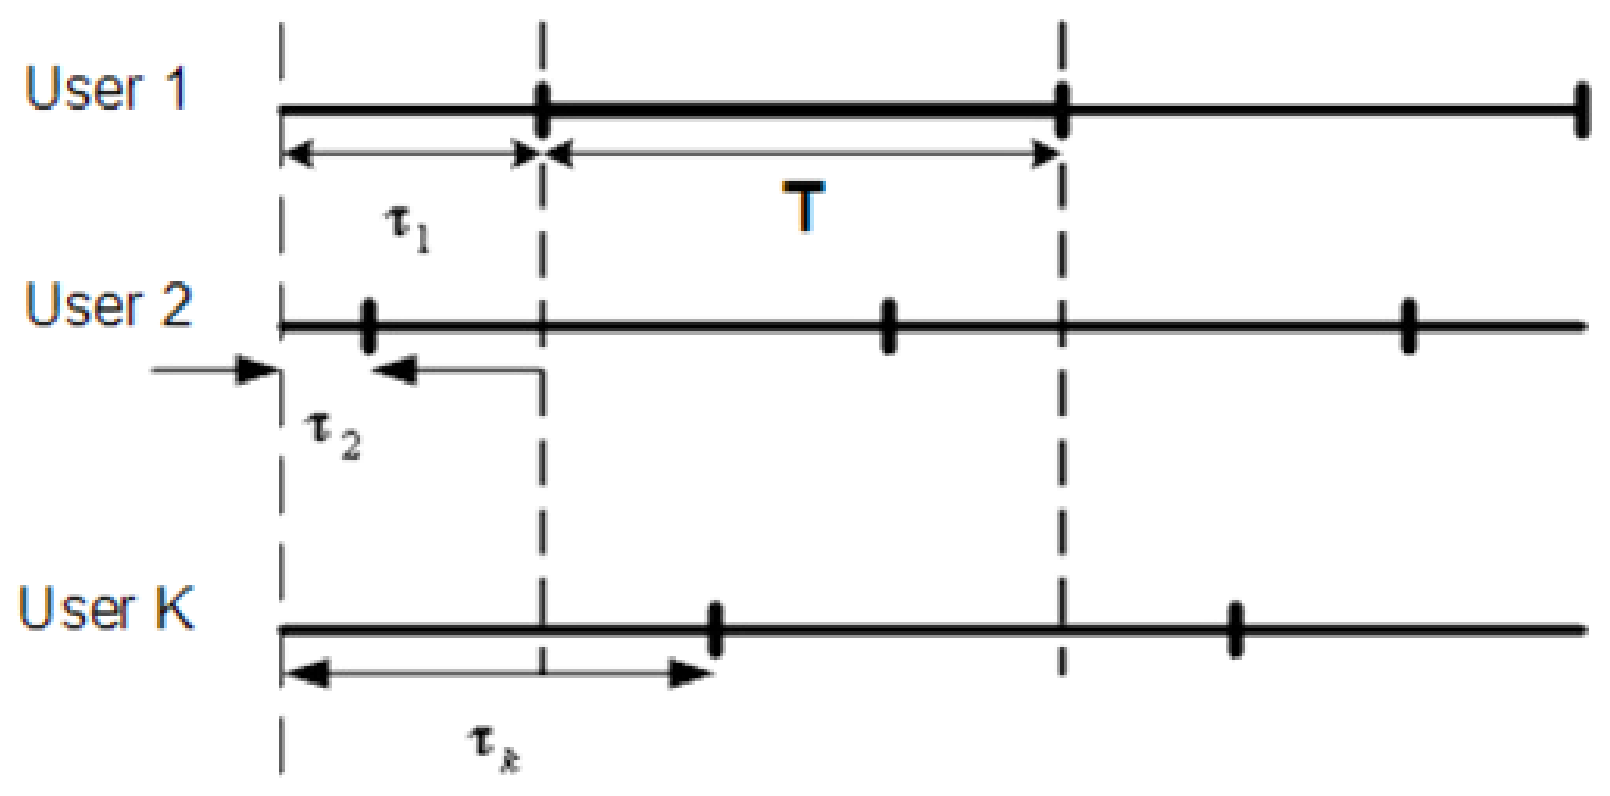
\includegraphics[width=4in]{AsynchCDMA.eps}}
\caption{Asynchronous multiuser channel
demonstration}\label{channel}
\end{figure}

\begin{equation}
\begin{array}{rcl}
\br_1&=&A_1b_1[n]\bs_1+\sum\limits_{k=2}^{K}A_k b_k[n-1]
\bs_{k_-}+\sum\limits_{k=2}^{K}A_k b_k[n] \bs_{k_+} + \bn
\end{array} \label{r}
\end{equation}

\noindent where $\bs_{k-}$ and $\bs_{k+}$ are named effective
signature sequences or part signature sequences that are
completely determined by the spreading sequences $\bs_k$ and the
delays relative to the first user $\tau_{k1}=\tau_k-\tau_1$.

When the received signal vector $\br$ is fed into a correlating
receiver bank that is matched to each user's spreading waveform,
the output signal vector can be expressed by

\begin{equation}
\begin{array}{rcl}
\by&=&\bR(1)\bA\bb[n-1]+\bR(0)\bA\bb[n]+\bR^{\rm
T}(1)\bA\bb[n+1]+\bar{\bn}
\end{array}
\end{equation}

\noindent where the zero-mean Gaussian process $\bar{\bn}$ has
autocovariance matrix

\begin{equation}
\begin{array}{rcl}
E\{\bar{\bn}_i\bar{\bn}_j^{\rm T}\}&=&\left\{
\begin{array}{ll}
\sigma^2\bR^{\rm T}(1)&j=i+1\\ \sigma^2\bR(0)&j=i\\
\sigma^2\bR(1)&j=i-1\\ \mathbf{0}&|j-i|>1
\end{array}\right.
\end{array}
\end{equation}

\noindent and the matrices $\bR(0)$ and $\bR(1)$ are defined by

\begin{equation}
\begin{array}{rcl}
R_{ij}(0)&=&\left\{
\begin{array}{ll}
1&j=i\\ \rho_{ij}&j<i\\ \rho_{ji}&j>i
\end{array}\right.
\end{array}
\end{equation}

\begin{equation}
\begin{array}{rcl}
R_{ij}(1)&=&\left\{
\begin{array}{ll}
0&j\geq i\\ \rho_{ij}&j<i
\end{array}\right.
\end{array}
\end{equation}

\subsection{Problem Description}

Multiuser detection is the techniques for mitigating the MAI at
either the base station or the mobile station. Most conventional
multiuser detection schemes assume the knowledge of the spreading
codes or channel parameters of the users that contribute to the
received signals for interference cancellation. In fact, it is
fair to assume that each mobile station has only knowledge of its
own spreading sequence and channel and the base station is only
aware of some knowledge of those in-cell active user, not
out-of-cell unknown interference. The blind multiuser detection,
which is designed to work only with the knowledge of the spreading
sequences and channel parameters of the concerned users, then is
more closed to practical applications. Compared with other
centralized schemes, linear blind multiuser detectors can be
implemented in a decentralized fashion where only the user or
users of interest need be demodulated. It was proposed by
Shnidman~\cite{Shni67} and is much closed to practical
applications. Most linear multiuser detectors for demodulating the
$k$th user's data bit in (\ref{r}) is in the form of a correlator
followed by a hard limiter, which could be expressed as

\begin{equation}
\begin{array}{rcl}
\hat{b}_k &=& \mbox{sign}\{\bw_k^{\rm T}\br\}
\end{array} \label{linear}
\end{equation}

\noindent where $\bw_k \in \mathbb{R}^{L\times 1}$ is the linear
representation of multiuser detector.

\pagebreak

\section{Blind Multiuser System Model And Detection Framework\label{BMUD_model}}

Most classic multiuser detection schemes assume knowledge of the
spreading waveform, amplitude and/or signal-to-noise ratios (SNR)
of all in-cell active users that contribute to received signals.
These receivers then exploit this knowledge to achieve optimal or
sub-optimal performance. These classic multiuser detectors have
comprehensively been investigated in~\cite{Verd98}. However, in
many practical situations, e.g. in the forward links of CDMA
mobile systems, it is difficult for the mobile station receivers
to known other existing users' information. So many blind
multiuser detectors are developed to operate without prior
knowledge regarding other users but using advanced signal
processing and estimation techniques to estimate other's
information or reconstruct signal/noise subspace. Instead of doing
this, we take a different approach for blind multiuser detection.
Here, instead of trying to restore other users' spreading sequence
information or estimate system statistical parameters, we propose
a new blind multiuser system model using a blind but "faked"
spreading matrix for the desired user(s). We say it is a blind but
"faked" spreading sequence matrix because

\begin{enumerate}

\item it only consists of the desired user's spreading sequence
and several previous received signal vector. No spreading sequence
or channel information regarding other users is involved.

\item it isn't a original spreading sequence matrix $\bS$ but
works like a spreading sequence matrix.

\end{enumerate}

\noindent We show that the desired user's information bits can be
detected based on this blind multiuser system model. In the
following, we present this novel blind multiuser system model and
detection framework. The major assumptions in our development are

\begin{enumerate}

\item The multiuser receiver structure is shown in Fig.
\ref{CDMA_links}. It is assumed that there are possible RAKE
receiver block and sequence estimation block before the MUD block
for each desired user. So, the practical spreading sequence
wave-form for each desired user is assumed to be known before MUD.
The same assumption is true for both forward and reverse links.

\item For each propagation path of interfering signals, if it
cannot be combined by RAKE, it may be taken as a different
interference user.

\end{enumerate}

\begin{figure}
\center{
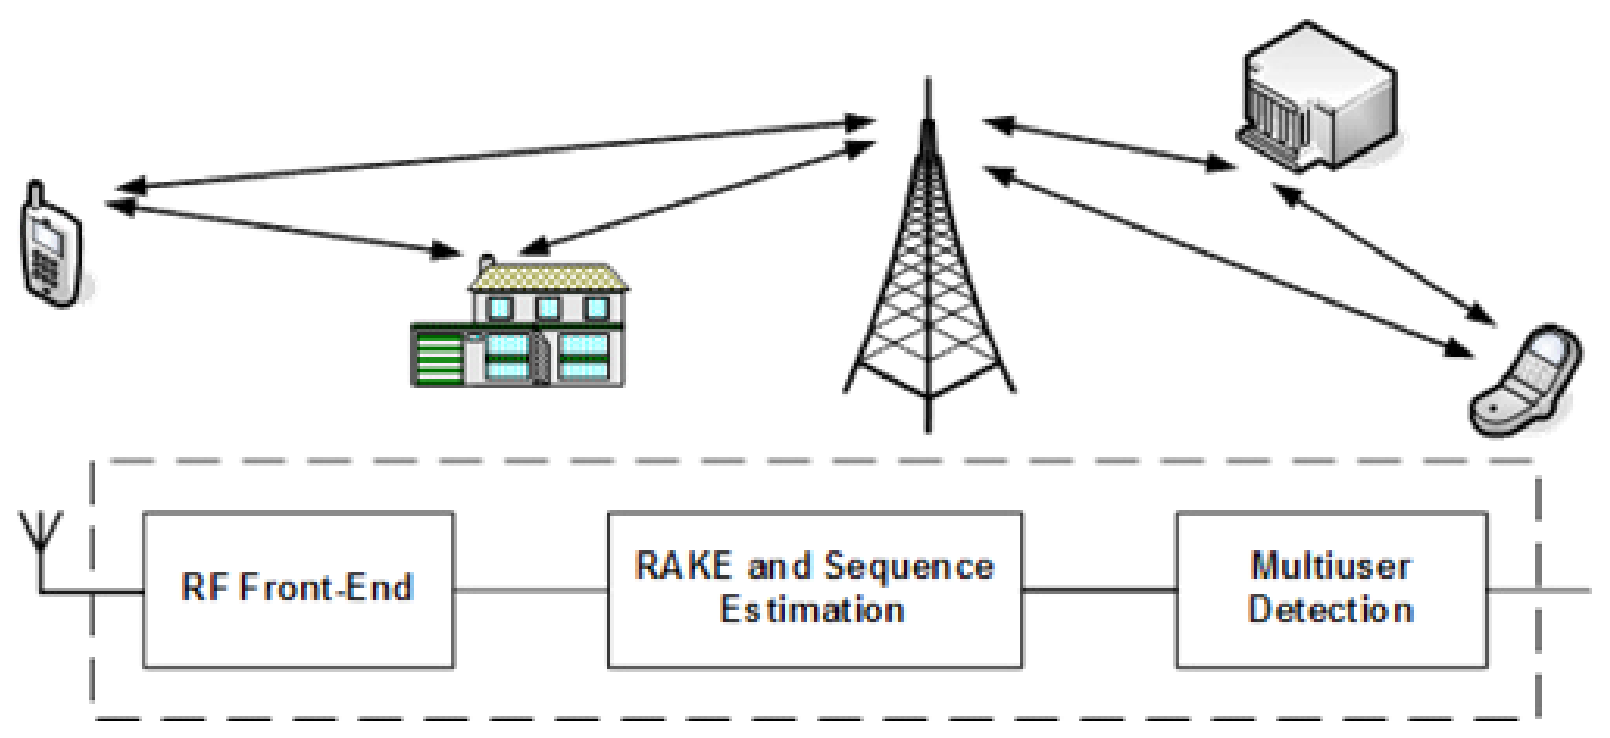
\includegraphics[width=5in]{CDMA_links.eps}}
\caption{A reverse link multiuser receiver}\label{CDMA_links}
\end{figure}



In this section, only the bits $b_1$ sent by the first user in a
synchronous CDMA system are considered. Blind multiuser detection
for asynchronous CDMA system and group-based CDMA systems will be
discussed in Section \ref{BMUD_mw_async} and \ref{GroupMUD}
individually.

\subsection{Blind Multiuser System Model}
At first we construct a new $L\times M$ blind spreading sequence
matrix $\bcS$ which is defined by

\begin{equation}
\begin{array}{rcl}
\bcS&=&[\matrix{\bar{\bs}_1&\bar{\bs}_2&\bar{\bs}_3&\ldots&\bar{\bs}_M}]\\
 &=&[\matrix{\bs_1&{\br}_{1}&{\br}_{2}&\ldots&{\br}_{M-1}}]\\
 &=&\left[\matrix{\bS\be_1&\bS{\bar\bb}_1&\bS{\bar\bb}_2&\ldots&\bS{\bar\bb}_{M-1}}\right] + {\bN}\\
 &=&\bS\left[\matrix{\be_1&{\bar\bb}_1&{\bar\bb}_2&\ldots&{\bar\bb}_{M-1}}\right] + {\bN}\\
 &=&\bS\left[\matrix{\be_1 & \bD }\right] + {\bN}\\
 &=&\bS\bB + {\bN}
\end{array} \label{S_0}
\end{equation}

\noindent where ${\br}_m$, $m=1,\ 2,\ \ldots,\ M-1$, are $M-1$
previously received independent vectors and the $K\times 1$ vector
${\bar\bb}_m=\left[\matrix{A_1b_1[m] & A_2b_2[m]& \ldots &
A_Kb_K[m]}\right]^{\rm T} = \bA\bb_m $ is the corresponding bit
vector for all $K$ users, $M\geq K$, $\bD = [{\bd}\
\tilde{\bD}^{\rm T}]^{\rm T}$ and the $(M-1)\times 1 $ vector
${\bd}$ is the known vector previously sent for the $1$st user,
${\bN}=[\mathbf{0}\ \tilde{\bN}]$ is a new noise matrix where the
first column is a zero vector and other columns are AWGN vectors
with the same distribution,

\begin{equation}
\begin{array}{rcl}
 \bB&=&\left[\matrix{\be_1 & \bD }\right]\\
  &=&\left[\matrix{\bg^{\rm T} \cr \matrix{\mathbf{0}& \tilde{\bD}}
 }\right]\\
 &=&\left[\matrix{\be_1 & \matrix{ {\bd}^{\rm T}\cr\tilde{\bD}} }\right]\\
 &=&\left[\matrix{1& \bd^{\rm T} \cr \mathbf{0}& \tilde{\bD}
 }\right]

\end{array}\label{B}
\end{equation}

\noindent is the information matrix associated with $\bcS$. $\bg =
\left[\matrix{1& \bd^{\rm T}}\right]^{\rm T}$ is a known
information vector for user 1, $\mbox{rank}\{\tilde{\bD}\}=K-1$
and $\mbox{rank}\{\bB\}=K$.

Combining (\ref{r_sync}) and (\ref{S_0}), the received signal
vector $\br$ can now be expressed by

\begin{equation}
\begin{array}{rcl}
\br&=&\bS\bA\bb + \bn\\
 &=&\bS\bB\bB^{+}\bar\bb + \bn\\
 &=&(\bcS-{\bN})\bB^{+}\bar\bb + \bn\\
 &=&\bcS\bB^{+}
 \bar\bb - {\bN}\bB^{+}\bar\bb + \bn\\
 &=&\bcS\bbf + \bar{\bn} \label{r_blind}
\end{array}
\end{equation}

\noindent where $\bB^{+} $ is the Moore-Penrose matrix inverse of
$\bB$ and the $K \times 1$ vector $\bbf$ is termed the detection
vector and defined by

\begin{equation}
\begin{array}{rcl}
\bbf&=&\left[\matrix{f_1\cr\tilde{\bbf}}\right]\\
 &=&\bB^{+}\bar\bb\\
 &=&\left[\matrix{\be_1&\bD}\right]^{+}\bar\bb\\
 &=&\left[\matrix{1&{\bd}^T\cr\mathbf{0}&\tilde{\bD}}\right]^{+}\left[\matrix{A_1b_1\cr\tilde{\bb}}\right]
\end{array} \label{DetectorVector}
\end{equation}

\noindent with the mean vector $\bm_{\bbf}=\bzero$ and the
covariance matrix $\bC_{\bbf}=\mbox{E}\left\{\bbf \bbf^{\rm
T}\right\}$, $\bar{\bn}$ is the new $L\times 1$ noise vector
defined by

\begin{equation}
\begin{array}{rcl}
\bar{\bn}&=&\bn-{\bN}\bB^{+}\bar\bb
\end{array} \label{new_noise}
\end{equation}

\noindent with mean vector $\bm_{\bar{\bn}}=\bzero$ and covariance
matrix

\begin{equation}
\begin{array}{rcl}
\bC_{\bar{\bn}}&=&\mbox{E}\left\{(\bn-{\bN}\bB^{+}\bar\bb)(\bn-{\bN}\bB^{+}\bar\bb)^{\rm T}\right\}\\
&=& \sigma^{2}\bI+\mbox{E}\left\{{\bN}\bC_{\bbf}{\bN}^{\rm
T}\right\}
\end{array} \label{var_n}
\end{equation}

\noindent and $\mbox{E}\left\{\cdot\right\}$ is the expectation
operator.


\subsection{Blind Multiuser Detection Framework}

Now, the classic multiuser detection model (\ref{r}) can be
replaced by (\ref{r_blind}) with $\bar{\bb}=\bA\bb$ being replaced
by the detection vector $\bbf$ in (\ref{DetectorVector}) and the
original AWGN vector $\bn$ being replaced by $\bar{\bn}$ in
(\ref{new_noise}). The comparison between the classic system model
and the proposed model is detailed in Tab.~\ref{ModelComp}.
Fortunately, the bit $b_1$ sent for user 1 can still be detected
using the detection vector $\bbf$ and the previously detected bit
vector $\bg$, which can be expressed by

\begin{equation}
\begin{array}{rcl}
\hat{b}_1 &=& \mbox{sign}\left\{\hat{A}_1\hat{b}_1\right\}\\
&=&\mbox{sign}\left\{\bg^{\rm T}\bbf\right\}\
\end{array} \label{b_estimation}
\end{equation}

\noindent and

\begin{equation}
\begin{array}{rcl}
\hat{A}_1 &=& \left|\hat{A}_1\hat{b}_1\right|\\
&=&\left|\bg^{\rm T}\bbf\right|\ .
\end{array} \label{A_estimation}
\end{equation}


\noindent The multiuser detection question for user $1$ now
becomes how to efficiently estimate $\bbf$ and construct $\bcS$
and $\bg$.


\begin{table}
\caption{Comparison between the class system model and the
proposed model}\label{ModelComp}
\begin{center}
\begin{tabular}{lcc}
Parameters&The proposed system model&The classic system model\\
\hline
Generality& Dedicated& Common\\
Input Vector &$\bbf\ -\ 1\times\rm M$&$\bb\ -\ 1\times\rm K$\\
Spreading Sequence Matrix &$\bcS\ -\ \rm L\times\rm M$&$\bS\ -\ \rm L\times\rm K$\\
Amplitude Matrix & N/A &$\bf{A}\ -\ \rm K\times\rm K$\\
Channel Noise Vector &$\bar\bn\ -\ 1\times\rm L$&$\bn\ -\ 1\times\rm L$\\
Output Vector&$\bf{r}\ -\ 1\times\rm L$&$\bf{r}\ -\ 1\times\rm L$\\
 \hline
\end{tabular}
\end{center}
\end{table}

\pagebreak


\section{Blind Multiuser Detectors\label{LBD}}

With (\ref{b_estimation}) and (\ref{A_estimation}), the proposed
blind multiuser detection framework can be illustrated in
Fig.~\ref{MUDstruct}. We can see that the performance of this
blind multiuser detection frame work highly depends on the
estimation of $\bbf$ and the accuracy of $\bg$. The estimation of
$\bbf$ actually is a typical linear estimation problem. In the
following, we discuss various algorithms for estimating $\bbf$
using different criteria, which including LS, BLU, MMSE criteria.
The formulations of different blind multiuser detectors are
presented following each estimation scheme.

\begin{figure}
\center{
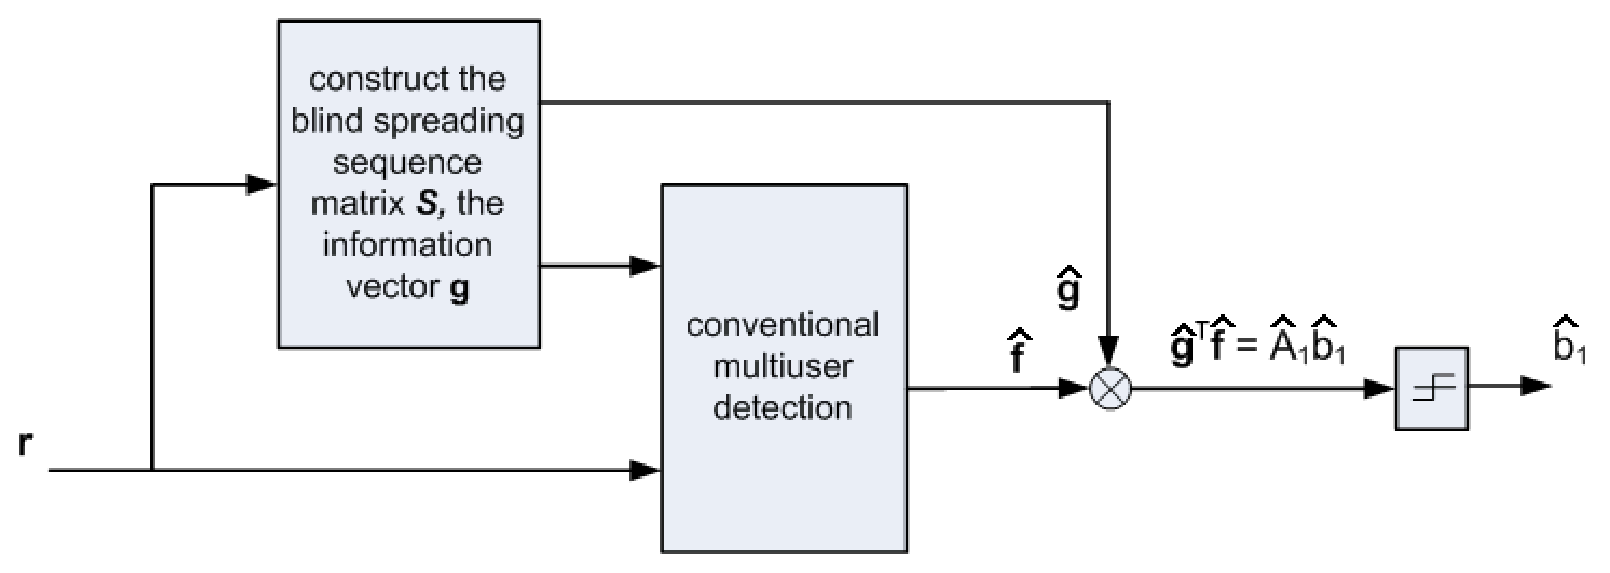
\includegraphics[width=6in]{BMUD_structure1.eps}
\caption{ The proposed blind multiuser detection structure.}
}\label{MUDstruct}
\end{figure}


\subsection{Least-Squares-Based Blind Detections}
Let us start from minimizing LS errors. LS-based algorithms are
widely used in practices because they are simple and easy to be
implemented. They only use signal models without any probabilistic
assumptions about data. The negative side, no claims about
optimality can be made and the statistical performance cannot be
assessed without some specific assumption about the probabilistic
structure of the data. According to the classic LS method, it is a
"best" fit scheme with minimizing the sum of squares of difference
between $\br$ and $\bcS\hat{\bbf}$. In a typical LS estimation
model, it normally assumes that the data matrix $\bcS$ is
error-free. Obviously this assumption cannot be true for our
proposed blind system model. Therefore, the LS, TLS and MLS blind
detections are proposed with different assumptions regarding
$\bcS$.

\subsubsection{Least Squares Detection }
At first, we assume that the measurements of $\bcS$ are assumed to
be free of error. All errors are confined to the received vector
$\br$. Hence, the detection vector can be estimated with solving
the following equation

\begin{equation}
\begin{array}{rcl}
{\bbf}_{\rm
LS}=\matrix{\mbox{arg}\min\limits_{\bx}\left\|\br-\bcS\bx\right\|_2}&\mbox{subject
to}&\br\subseteq \mbox{span}\{\bcS\}
\end{array}
\label{LSProb}
\end{equation}

Suppose $\bU^T\bcS\bV=\mathbf{\Sigma}$ is the SVD of
$\bcS\in\mathbb{R}^{L\times
 K}$ with $r=\mbox{rank}(\bcS)$. And if $\bU=[\matrix{\bu_1&\bu_2&\ldots&\bu_L}]$,
 $\bV=[\matrix{\bv_1&\bv_2&\ldots&\bv_K}]$, $\mathbf{\Sigma}=\mbox{diag}\{[\matrix{\sigma_1&\ldots\sigma_r&0&\ldots&0}]\}$ and $\br\in \mathbb{R}^{L\times 1}$,
 then LS estimation of $\bbf$ is

 \begin{equation}
 \begin{array}{rcccl}
 \matrix{\bbf_{\rm
 LS}&=&\sum\limits_{i=1}^{r}\frac{\bu_i^{\rm T}\br}{\sigma_i}\bv_i&=&\bcS^+\br}&=&\bbf + \bcS^+\bar{\bn}
 \end{array}\label{f_LS}
 \end{equation}

\noindent which minimizes $\|\bcS\bd-\br\|_2$ and has the smallest
2-norm of all minimizers. Moreover
 \begin{equation}
 \matrix{\varepsilon_{\rm LS}^2 &=& \min\limits_{\bx\in\mathbb{R}}\|\bcS\bx-\br\|_2^2 &=& \sum\limits_{i=r+1}^{L}(\bu_i^{\rm T}\br)^2}
 \end{equation}

\noindent The linear filter representation of the LS detector can
be written by

\begin{equation}
\begin{array}{rcl}
\bw_{\rm LS}&=&\bcS^{+\rm T}\bg
\end{array} \label{w_LS}
\end{equation}

\noindent and the information bit of user 1 can be detected by

\begin{equation}
\begin{array}{rcl}
\hat{b}_1&=&\mbox{sign}\left\{\bw_{\rm LS}^{\rm T}\br\right\}\\
&=&\mbox{sign}\left\{\bg^{\rm T}\bcS^{+}\br\right\}
\end{array} \label{w_LS}
\end{equation}



\subsubsection{Total Least Squares Estimation}

It assume $\bcS$ to be error-free in the previous LS estimate of
the detection vector $\bbf$. However, this assumption is not
entirely accurate according to the definition of $\bcS$ in
(\ref{S}) since there is a noise term, $\bN$. On the other hand,
$\br$ can also be expressed as
\begin{equation}
\begin{array}{rcl}
\br&=&(\bcS-\bN)\bB^{+}\bb + \bn\\
 &=&\hat{\bcS}\bd + \bn
\end{array}
\end{equation}
where  $\hat{\bcS}=\bcS-\bN=\bS\bB$.  The minimization problem of
(\ref{LSProb}) can then be transformed into the following TLS
problem:
\begin{equation}
\begin{array}{rcl}
\left[\bcS_{\rm TLS},\ \bbf_{\rm
TLS}\right]&=&\matrix{\mbox{arg}\min\limits_{\bar{\bcS},\
\bx}\left\|\left[ \matrix{\bcS&\br} \right] - \left[
\matrix{\bar{\bcS}& \bar{\bcS}\bx}\right]\right\|_2}
\end{array},
\label{TLSProb}
\end{equation}
subject to $\br\subseteq\mathbb{R}(\bar{\bcS})$.

 Let $\bcS=\bU^{'}\mathbf{\Sigma}^{'}\bV^{'\rm T}$ and
$[\bcS\ \br]=\bU\mathbf{\Sigma}\bV^{\rm T}$ be the SVD of $\bcS$
and $[\bcS\ \br]$, respectively. If $\sigma_K^{'}
> \sigma_{K+1}$, TLS estimation of $\bbf$ then is
\begin{equation}
\bbf_{\rm TLS} = \left(\bcS^{\rm
T}\bcS-\sigma_{K+1}^2\bI\right)^{-1}\bcS^{\rm T}\br
\end{equation}
and
\begin{equation}
\begin{array}{rcl}
\varepsilon_{\rm TLS}^{2}&=&\min\limits_{\bx\in
\mathbb{R}^{K\times
1}}\|\bcS\bx-\br\|_2^2 \\
 &=& \sigma_{K+1}^2\left[1+\sum_{i+1}^{K}\frac{\left(\bu_i^{'\rm T}\br\right)^2}
{\sigma_i^{'2}-\sigma_{K+1}^2}\right]
\end{array}
\end{equation}
where $\bU=[\bu_1\ \bu_2\ \ldots\ \bu_L]$, $\bV=[\bv_1\ \bv_2\
\ldots\ \bv_{K+1}]$, $\mathbf{\Sigma}={\rm diag}\{[\sigma_1\
\sigma_2 \ldots\ \sigma_{K+\min\limits\{L-K,\ 1\}}]\}$ and
$\bU^{'}=[\bu_1^{'}\ \bu_2^{'}\ \ldots\ \bu_L^{'}]$,
 $\bV^{'}=[\bv_1^{'}\ \bv_2^{'}\ \ldots\ \bv_{K}^{'}]$,
 $\mathbf{\Sigma}^{'}={\rm diag}\{[\sigma_1^{'}\ \sigma_2^{'}\ \ldots\
 \sigma_K^{'}]\}$. And the linear filter $\bw_{\rm TLS}$ is

\begin{equation}
\begin{array}{rcl}
\bw_{\rm TLS}&=&\bcS(\bcS^{\rm T}\bcS-\sigma_{K+1}^2\bI)^{-1}\bg
\end{array}\label{w_TLS}
\end{equation}

\noindent and the information bit of user 1 can be detected by

\begin{equation}
\begin{array}{rcl}
\hat{b}_1&=&\mbox{sign}\left\{\bw_{\rm TLS}^{\rm T}\br\right\}\\
&=&\mbox{sign}\left\{\bg^{\rm T}(\bcS^{\rm
T}\bcS-\sigma_{K+1}^2\bI)^{-1}\bcS^{\rm T}\br\right\}
\end{array} \label{w_LS}
\end{equation}


\subsubsection{Mixed LS/TLS Detection}

In the LS problem of (\ref{LSProb}), it assumed the blind
signature matrix $\bcS$ is error-free. Again, this assumption is
not completely accurate. In the TLS problem of (\ref{TLSProb}), it
assumed that in each column of the blind signature matrix, $\bcS$,
some noise or error exists.  This assumption also is not complete.
Though there exists a noise or error matrix $\bN$ in $\bcS$ from
(\ref{S}), its first column is exactly known to be noise-free or
error-free.  Hence, to maximize the estimation accuracy of the
detection vector $\bbf$, it is natural to require that the
corresponding columns of $\bcS$ be unperturbed since they are
known exactly. The problem  of estimating the detection vector
$\bd$ can then be transformed into the following MLS problem by
considering (\ref{LSProb}) and (\ref{TLSProb}):
\begin{equation}
\begin{array}{rcl}
\left[\bcS_{\rm MLS},\ \bbf_{\rm MLS}\right] &=
&\matrix{\mbox{arg}\min\limits_{\bar{\bcS},\
\bx}\left\|\left[\matrix{\tilde{\bcS}&\br}\right]-\left[\matrix{\bar{\bcS}&[\bs_1\
 \bar{\bcS}]\bx}\right]\right\|_{2} }
\end{array}\label{MLSProb}
\end{equation}
subject to $\br\subseteq\mbox{span}\left\{[\bs_1\
\bar{\bcS}]\right\}$. The following lemma outlines the MLS
solution.

Consider the MLS problem in (\ref{MLSProb}) and perform the
Householder transformation $\bQ$ on the matrix
$[\matrix{\bcS&\br}]$ so that
\begin{equation}
\begin{array}{rcl}
\bQ^{\rm
T}[\matrix{\bs_1&\bar{\bcS}&\br}]&=&\left[\matrix{R_{11}&\bR_{12}&R_{1r}\cr
\mathbf{0}&\bR_{22}&\bR_{2r}}\right]
\end{array}
\end{equation}
where $R_{11}= A_1$, $\bR_{12}$ is a $1\times (M-1)$ vector,
$\bR_{22}$ is a $(L-1)\times (M-1)$ matrix and $\bR_{2r}$ is a
$(L-1)\times 1$ vector and

\begin{equation}
\begin{array}{rcl}
\bQ &=&\bI - \frac{1}{A_1(A_1-s_{11})}\left[\matrix{s_{11}-A_1\cr
s_{12}\cr \vdots \cr s_{1L}}\right]\left[\matrix{(s_{11}-A_1)&
s_{12}& \cdots & s_{1L}}\right]
\end{array}
\end{equation}



Denote $\sigma'$ as the smallest singular value of $\bR_{22}$ and
$\sigma$ as the smallest singular value of
$[\matrix{\bR_{22}&\bR_{2r}}]$. If $\sigma'>\sigma$, then the MLS
solution uniquely exists and is given by
\begin{equation}
\begin{array}{rcl}
\bbf_{\rm MLS}&=&\left(\bcS^{\rm
T}\bcS-\sigma^2\left[\matrix{0&\mathbf{0}\cr\mathbf{0}&\mathbf{I}_{M-1}}\right]\right)^{-1}\bcS^{\rm
T}\br
\end{array}.
\end{equation}

\noindent The linear filter representation of this MLS detection
is

\begin{equation}
\begin{array}{rcl}
\bw_{\rm MLS}&=&\bcS\left(\bcS^{\rm
T}\bcS-\sigma^2\left[\matrix{0&\mathbf{0}\cr\mathbf{0}&\mathbf{I}_{M-1}}\right]\right)^{-1}\bg
\end{array} \label{w_MLS}
\end{equation}


\noindent and the information bit of user 1 can be detected by

\begin{equation}
\begin{array}{rcl}
\hat{b}_1&=&\mbox{sign}\left\{\bw_{\rm MLS}^{\rm T}\br\right\}\\
&=&\mbox{sign}\left\{\bg^{\rm T}\left(\bcS^{\rm
T}\bcS-\sigma^2\left[\matrix{0&\mathbf{0}\cr\mathbf{0}&\mathbf{I}_{M-1}}\right]\right)^{-1}\bcS^{\rm
T}\br\right\}
\end{array} \label{w_LS}
\end{equation}


\subsection{Best Linear Unbiased Detection}

We begin by assuming the linear structure

\begin{equation}
\begin{array}{rcl}
{\bbf}_{\rm BLU}&=&\bW_{\rm BLU}^{\rm T}\br
\end{array}
\end{equation}

\noindent for this so-called best linear unbiased estimator
(BLUE). Matrix $\bW_{\rm BLU}$ is designed such that:

\begin{enumerate}

\item $\bcS$ must be deterministic,

\item $\bar{\bn}$ must be zero mean with positive definite known
covariance matrix $\bC_{\bar{\bn}}$,

\item ${\bbf}_{\rm BLU}$ is an unbiased estimator of $\bbf$,

\item and the error variance for each of the $M$ parameters is
minimized as

\begin{equation}
\begin{array}{rcl}
\bW_{\rm BLU}&=&\min\limits_{\bW_{\bbf}}
\mbox{var}\left\{\bW_{\bbf}^{\rm T}\br\right\}
\end{array}
\end{equation}


\end{enumerate}

In this way, ${\bbf}_{\rm BLU}$ will be unbiased and efficient,
within the class of linear estimators, by design. The resulting
best linear unbiased estimator is (Gauss-Markov Theorem):

\begin{equation}
\begin{array}{rcl}
{\bW}_{\rm BLU}&=&\bC_{\bar{\bn}}^{-1}\bcS(\bcS^{\rm
T}\bC_{\bar{\bn}}^{-1}\bcS)^{-1}
\end{array}
\end{equation}

\noindent and

\begin{equation}
\begin{array}{rcl}
{\bbf}_{\rm BLU}&=&\bW_{\rm BLU}^{\rm T}\br\\
 &=&(\bcS^{\rm
T}\bC_{\bar{\bn}}^{-1}\bcS)^{-1}\bcS^{\rm
T}\bC_{\bar{\bn}}^{-1}\br\ .
\end{array} \label{BLUE}
\end{equation}

\noindent The covariance matrix of ${\bbf}_{\rm BLU}$ given by

\begin{equation}
\begin{array}{rcl}
{\bC}_{\bbf_{\rm BLU}}&=&(\bcS^{\rm
T}\bC_{\bar{\bn}}^{-1}\bcS)^{-1}
\end{array}.
\end{equation}

\noindent Since the above data are of Gaussian distributions, the
BLUE in (\ref{BLUE}) is also the minimum variance unbiased
estimation. The linear filter representation of this detector is

\begin{equation}
\begin{array}{rcl}
{\bw}_{\rm BLU}$=$\bC_{\bar{\bn}}^{-T}\bcS(\bcS^{\rm
T}\bC_{\bar{\bn}}^{-1}\bcS)^{-1}\bg
\end{array}.\label{w_BLU}
\end{equation}

\noindent Now the question is how we know about
$\bC_{\bar{\bn}}^{-1}$. With (\ref{var_n}), $\bC_{\bar{\bn}}^{-1}$
can be decided by $\sigma^2$ and $\bC_{\bbf}$. Let us consider
$\bC_{\bbf}$ first. Though the PDF of $\bB$ may be determined, the
PDF of $\bB^{+}$ is largely unknown. This makes it is hard to
calculate the closed-form solution of $\bC_{\bbf}$ and
$\bC_{\tilde{\bn}}$. However, with Girko's Law, when
$\alpha=(K-1)/(M-1)$ is fixed, $K$, $M$ $\rightarrow\infty$, the
diagonal element of
$\frac{1}{M-1}\tilde{\bD}^+\tilde{\bb}\tilde{\bb}^{\rm
T}\tilde{\bD}^{\rm +T}$ may be approximated
by~\cite{Muller,Hanly90}

\begin{equation}
\begin{array}{rcl}
\lim\frac{1}{M-1}\left[\tilde{\bD}^+\tilde{\bb}\tilde{\bb}^{\rm
T}\tilde{\bD}^{\rm +T}\right]_{ii}^{-1}&=&1-\alpha
\end{array}.
\end{equation}

\noindent So, $\bC_{\bbf}$ can be approximated by

\begin{equation}
\begin{array}{rcl}
\bC_{\bbf}&=&\mbox{E}\left\{\bbf\bbf^{\rm T}\right\}\\
&=&\mbox{E}\left\{\left[\matrix{(A_1b_1-\bd^{\rm
T}\tilde{\bD}^{\rm +}\tilde{\bb})^2&(A_1b_1-\bd^{\rm
T}\tilde{\bD}^{\rm +}\tilde{\bb})\tilde{\bb}^{\rm
T}\tilde{\bD}^{\rm +T}\cr (A_1b_1-\bd^{\rm T}\tilde{\bD}^{\rm
+}\tilde{\bb})\tilde{\bD}^+\tilde{\bb}&
\tilde{\bD}^+\tilde{\bb}\tilde{\bb}^{\rm T}\tilde{\bD}^{\rm
+T}}\right]\right\}\\
&\approx&\left[\matrix{\frac{2M-K-1}{M-K}A_1^2&\bzero^{\rm
T}\cr\bzero&\frac{1}{M-K}\bI}\right]
\end{array}
\end{equation}

\noindent and

\begin{equation}
\begin{array}{rcl}
\bC_{\bar\bn}&=&\sigma^{2}\bI+\mbox{E}\left\{{\bN}\bC_{\bbf}{\bN}^{\rm
T}\right\}\\
&=&\sigma^{2}\frac{2M-K-1}{M-K}\bI
\end{array}
\end{equation}


Thus, the linear filter representation of the BLU detector can be
approximated by


\begin{equation}
\begin{array}{rcl}
{\bw}_{\rm BLU}&=&\bcS(\bcS^{\rm T}\bcS)^{-1}\bg
\end{array}\label{w_BLUE_approx}
\end{equation}


\noindent and the information bit of user 1 can be detected by

\begin{equation}
\begin{array}{rcl}
\hat{b}_1&=&\mbox{sign}\left\{\bw_{\rm TLS}^{\rm T}\br\right\}\\
&=&\mbox{sign}\left\{\bg^{\rm T}(\bcS^{\rm T}\bcS)^{-1}\bcS^{\rm
T}\br\right\}
\end{array}
\end{equation}



\subsection{Minimum Mean Square Detection}
Now we propose a linear estimator based on MMSE criterion. This
class of estimators are generically termed Wiener filter. Given
measurements $\br$, the MSE estimator of $\bbf$, ${\bbf}_{\rm MS}
= f( \br )$, minimizes the mean-squared error $J_{\rm
MSE}=E\{||\bbf-\hat{\bbf}||_2^2\}$. The function $f(\br)$ may be
nonlinear or linear and its exact structure is determined by
minimizing $J_{\rm MSE}$. When $\bbf$ and $\br$ are jointly
Gaussian, the linear estimator $\bW_{\rm MMS}$ that minimizes the
mean-sqared error is (Bayesian Gauss-Markov Theorem)

\begin{equation}
\begin{array}{rcl}
{\bW}_{\rm MMS} &=&
\bC_{\bar{\bn}}^{-1}\bcS(\bC_{\bbf}^{-1}+\bcS^{\rm
T}\bC_{\bar{\bn}}^{-1}\bcS)^{-1}
\end{array}\label{W_MSE}
\end{equation}

\noindent and

\begin{equation}
\begin{array}{rcccl}
{\bbf}_{\rm MMS} &=&{\bW}_{\rm MS}^{\rm T}\br
&=&(\bC_{\bbf}^{-1}+\bcS^{\rm
T}\bC_{\bar{\bn}}^{-1}\bcS)^{-1}\bcS^{\rm
T}\bC_{\bar{\bn}}^{-1}\br
\end{array}. \label{MSE}
\end{equation}

\noindent The performance of the linear MMSE estimator is measured
by the error vector $\mathbf{\varepsilon_{\rm MS}}=\bbf-\bbf_{\rm
MS}$ whose mean is zero and covariance matrix is

\begin{equation}
\begin{array}{rcl}
\bC_{\mathbf{\varepsilon_{\rm MMS}}} &=&
(\bC_{\bbf}^{-1}+\bcS^{\rm T}\bC_{\bar{\bn}}^{-1}\bcS)^{-1}
\end{array}.
\end{equation}

The linear filter representation of the blind linear MMSE detector
with $\bbf_{\rm MS}$ is

\begin{equation}
\begin{array}{rcl}
{\bw}_{\rm MMS}&=& \bC_{\bar{\bn}}^{-\rm
T}\bcS(\bC_{\bbf}^{-1}+\bcS^{\rm
T}\bC_{\bar{\bn}}^{-1}\bcS)^{-1}\bg
\end{array} \label{w_MSE}
\end{equation}

\noindent and the information bit of user 1 can be detected by

\begin{equation}
\begin{array}{rcl}
\hat{b}_1&=&\mbox{sign}\left\{\bw_{\rm TLS}^{\rm T}\br\right\}\\
&=&\mbox{sign}\left\{\bg^{\rm T}(\bC_{\bbf}^{-1}+\bcS^{\rm
T}\bC_{\bar{\bn}}^{-1}\bcS)^{-1}\bcS^{\rm
T}\bC_{\bar{\bn}}^{-1}\br\right\}
\end{array}
\end{equation}


\pagebreak

\section{Multi-Window Asynchronous Blind Multiuser Detection\label{BMUD_mw_async}}
For asynchronous cases, Verd\'{u} suggested to use a one-shot
version of his decorrelating detector, the truncated-window
decorrelating detector of single window length, in which
$1+2(K-1)=2K-1$ filters, where $K$ is the number of users, are
matched to one full code of a specific user (without loss of
generality, called the first user) and two filters matched to each
of the other users. One filter is matched to the \textquotedblleft
previous\textquotedblright\ part of its code, corresponding to the
time between zero and $\tau_k$, where $\tau_k$ is the delay of
user $k$ with respect to the first user, and to the
\textquotedblleft current\textquotedblright\ part of the code,
corresponding to the time between $\tau_k$ and $T$. In this case,
it not only requires the information about other active users'
signature but also the time delay of other users with respect to
the desired user. Furthermore, since only the signature
information of the other users is spared in a signature matrix of
the nearly doubled size, the performance of this one-short
decorrelating detector is worse than the complete asynchronouse
decorrelating detector in terms of both bit-error rate (BER) and
near-far resistance (NFR)~\cite{Verd98}. Here, a multiple-windowed
scheme is proposed instead. Without loss of the generality, we
show the detection of the bits sent by user $1$ at $P$ consecutive
time intervals $t=n-P+1$, $n-P+2$, $\ldots$, $n$, where $P$ is the
size of the detection window. And the $P$ consecutive information
bits in the signal vector $\bb_1$ will be simultaneously detected.
For this, a new $PL\times M$ blind signature matrix $\bcS$ is
defined by


\begin{equation}
\begin{array}{rcl}
\bcS&=&[\matrix{\bar{\bs}_1&\bar{\bs}_2&\bar{\bs}_3&\ldots&\bar{\bs}_M}]\\
 &=&[\matrix{\bI_P \otimes\bs_1&{\br}_{1}&{\br}_{2}&\ldots&{\br}_{M-P}}]\\
 &=&\left[\matrix{\bS\bE_p&\bS\bar{\bb}_1&\bS\bar{\bb}_2&\ldots&\bS\bar{\bb}_{M-P}}\right]+ {\bN}\\
 &=&\bS\left[\matrix{\bE_p&\bar{\bb}_1&\bar{\bb}_2&\ldots&\bar{\bb}_{M-P}}\right]+ {\bN}\\
 &=&\bS\left[\matrix{\bE_p & \bD }\right]+ {\bN}\\
 &=&\bS\bB + {\bN}
\end{array} \label{S}
\end{equation}

\noindent where $\bS$ becomes
$\left[\matrix{\bar{\bS}_1&\bar{\bS}_2&\bar{\bS}_3&\ldots&\bar{\bS}_K}\right]$
is a $PL\times (PK+K-1)$ matrix with

\begin{equation}
\begin{array}{rclcl}
\bar{\bS}_1&=&\bI_P\otimes\bs_1
&=&\mbox{diag}\left\{\matrix{\bs_1&\bs_1&\ldots&\bs_1}\right\}_{PL\times
P}
\end{array},
\end{equation}

\begin{equation}
\begin{array}{rcl}
\bar{\bS}_k&=&\mbox{diag}\left\{\matrix{\bs_{k-}&\bs_k&\ldots&\bs_k&\bs_{k+}}\right\}_{PL\times
(P+1)}
\end{array},
\end{equation}

\begin{equation}
\begin{array}{rcl}
\bB&=&\left[\matrix{\bE&\bar\bb_1&\ldots&\bar\bb_{M-P}}\right]
\end{array},
\end{equation}

\begin{equation}
\begin{array}{rcl}
\bE_p&=&\left[\matrix{\bI_P&\mathbf{0}}\right]^{\rm T}
\end{array},
\end{equation}


\begin{equation}
\begin{array}{rcl}
\bA&=&\mbox{diag}\left\{\matrix{\bA_1&\bA_2&\ldots&\bA_K}\right\}
\end{array},
\end{equation}

\begin{equation}
\begin{array}{rcl}
\bA_1&=&\mbox{diag}\left\{\matrix{A_1&A_1&\ldots&A_1}\right\}_{P\times
P}
\end{array},
\end{equation}

\begin{equation}
\begin{array}{rcl}
\bA_k&=&\mbox{diag}\left\{\matrix{A_k&A_k&\ldots&A_k}\right\}_{(P+1)\times
(P+1)}
\end{array},
\end{equation}

\begin{equation}
\begin{array}{rcl}
\bar\bb_m&=&\bA\bb_m
\end{array},
\end{equation}

\begin{equation}
\begin{array}{rcl}
\bb_m&=&\left[\matrix{\bb_{1m}^{\rm T}&\bb_{2m}^{\rm
T}&\ldots&\bb_{Km}^{\rm T}}\right]^{\rm T}
\end{array},
\end{equation}

\begin{equation}
\begin{array}{rcl}
\bb_{1m}&=&\left[\matrix{b_{1}[m-P+1]&\ldots&b_{1}[m]}\right]^{\rm
T}
\end{array},
\end{equation}

\begin{equation}
\begin{array}{rcl}
\bb_{km}&=&\left[\matrix{b_{k}[m-P]&b_{k}[m-P+1]&\ldots&b_{k}[m]}\right]^{\rm
T}
\end{array}
\end{equation}


\noindent where $\otimes$ denotes the Kronecker product, $vec$
denotes the stacking operation, $k=2,\ 3,\ \ldots,\ K$, ${\br}_i$
with $i=1,\ 2,\ \ldots,\ M-P$ are the previously received vectors,
the $(PK+K-1) \times 1$ vector $\bar{\bb}_i$ is the corresponding
information vector which includes $P$ consecutive bits sent by the
desired user and $(P+1)$ consecutive bits sent by the other $K-1$
users, $\bD = [\bar{\bD}^{\rm T}\ \tilde{\bD}^{\rm T}]^{\rm T}$.
The $(M-P)\times P$ vector $\bar{\bD}$ is the bit vector
consisting of the known bits sent by the desired user before.
$\mbox{rank}\{\tilde{\bD}\}=PK+K-P-1$, ${\bN}=[\mathbf{0}\
\tilde{\bN}]$ and

\begin{equation}
\begin{array}{rcccccl}
 \bB&=&\left[\matrix{\bE_p &{\bD} }\right]
 &=&\left[\matrix{\bG_p \cr \matrix{\mathbf{0}& \tilde{\bD}}
 }\right]
 &=&\left[\matrix{\bI_P& \bar{\bD} \cr \mathbf{0}& \tilde{\bD} }\right]

\end{array}\label{B_p}
\end{equation}

\noindent and $\mbox{rank}\left\{\bB\right\}=PK+K-1$.

With (\ref{r}) and (\ref{S}), the relationship between the
received signal vector $\br_p$, whose length is $PL$, and the new
blind signature matrix $\bcS$ can be expressed as\footnote{Without
loss of the generality, we drop the subscript $1$ for user $1$.}

\begin{equation}
\begin{array}{rcl}
\br_p&=&\bS\bA\bb + \bn\\
 &=&\bS\bB\bB^{+}\bar\bb + \bn\\
 &=&(\bcS-{\bN})\bB^{+}\bar\bb + \bn\\
 &=&\bcS\bB^{+}\bb-\bar{\bN}\bB^{+}\bb + \bn\\
 &=&\bcS\bbf + \bar{\bn} \label{rn}
\end{array}
\end{equation}

\noindent where the notations $\br$, $\bcS$, $\bS$, $\bbf$,
$\ldots$ share the same definitions in Section \ref{BMUD_model}
but each of them is expanded in time-domain. Also, it is very
straightforward to prove that the bits vector $\bb_1$ which
consists of $P$ bits sent by User 1 at the consecutive time
intervals $t=n-P+1$, $n-P+2$, $\ldots$, $n$ can be estimated using
the following conclusion.

\begin{lemma}
The bit vector $\bb_1$ sent for the first user at the consecutive
time intervals $t=n-P+1$, $n-P+2$, $\ldots$, $n$ can be detected
by
\begin{equation}
\begin{array}{rcl}
\hat{\bb}_1&=&\mbox{sign}\left\{\hat{A}_1\hat{\bb}_1\right\}\\
&=&\mbox{sign}\left\{\bG_p\bbf\right\}
\end{array}\label{bb_estimate}
\end{equation}

\end{lemma}


\begin{proof}

At first, $\bb_1$ can be estimated by
\begin{equation}
\begin{array}{rcl}
\hat{\bb}_1&=&\mbox{sign}\left\{A_1\bb_1-{\bar{\bD}}\tilde{\bD}^{+}\tilde{\bb}+{\bar{\bD}}\tilde{\bD}^{+}\tilde{\bb}\right\}\\
&=&
\mbox{sign}\left\{\left[\matrix{\bI_p&{\bar\bD}}\right]\left[\matrix{A_1\bb_1-{\bar\bD}\tilde{\bD}^{+}\tilde{\bb}\cr\tilde{\bD}^{+}\tilde{\bb}}\right]\right\}\\
&=& \mbox{sign}\left\{\bG_p\left[\matrix{\bI_p&-{\bar\bD}\tilde{\bD}^{+}\cr\bzero&\tilde{\bD}^{+}}\right]\left[\matrix{A_1\bb_1\cr\tilde{\bb}}\right]\right\}\\
&=&
\mbox{sign}\left\{\bG_p\left[\matrix{\bI_p&-{\bar\bD}\tilde{\bD}^{+}\cr\bzero&\tilde{\bD}^{+}}\right]\bar\bb\right\}
\end{array}\label{bb1}
\end{equation}


\noindent On the other hand, with (\ref{B_p}), we know that

\begin{equation}
\bB\left[\bE_p\
\matrix{-{\bar\bD}\tilde{\bD}^+\cr\tilde{\bD}^+}\right]\bB
=\left[\matrix{\bI_p&{\bar\bD}\cr\bzero&\tilde{\bD}}\right]\left[\matrix{\bI_p&-{\bar\bD}\tilde{\bD}^+\cr\bzero&\tilde{\bD}^+}\right]\left[\matrix{\bI_p&{\bar\bD}\cr\bzero&\tilde{\bD}}\right]
=\bB\ . \label{psedoB1_p}
\end{equation}

\noindent So, the Moore-Penrose Matrix inverse $\bB^{+}$ of $\bB$
can be written by

\begin{equation}
\bB^{+}
=\left[\matrix{\bI_p&-{\bar\bD}\tilde{\bD}^+\cr\bzero&\tilde{\bD}^+}\right]\
. \label{psedoB2_p}
\end{equation}


\noindent Using (\ref{B_p}) and (\ref{psedoB2_p}), (\ref{bb1}) can
be re-written by

\begin{equation}
\begin{array}{rcl}
\hat{\bb}_1&=& \mbox{sign}\left\{\bG_p\bB^{+}\bb\right\}\\
&=& \mbox{sign}\left\{\bG_p\bbf\right\}\\
\end{array}
\end{equation}

\noindent and the detection vector $\bbf$ can be re-written by

\begin{equation}
\begin{array}{rcl}
\bbf&=&\left[\matrix{A_1\bb_1-{\bar\bD}\tilde{\bD}^{+}\tilde{\bb}\cr\tilde{\bD}^{+}\tilde{\bb}}\right]
\end{array} \label{DetectorVector2_asynch}
\end{equation}


This lemma is then proven.
\end{proof}


\pagebreak




\section{Group-Wised Blind Multiuser Detection\label{GroupMUD}}
The concept of group-based multiuser detection was originally
introduced for designing low-complexity and suboptimal multiuser
detectors with partition all active users into several disjoint
smaller-sized groups. Normally these group detectors operate
parallelly while each group detector uses the decision of other
groups to do interference cancellations in a sequential
style~\cite{Mahesh95}. Recently, this concept is extended for
multiuser detection with the separation of in-cell users and
out-of-cell users at the base station of CDMA
system~\cite{Wang99A}, since both base station and mobile station
can receive in-cell signals and out-of-cell interference as in
Fig. \ref{CDMA_grouplinks}. It can be used help both decrease the
computation complexity of multiuser receiver and improve its
performance.

\begin{figure}
\center{
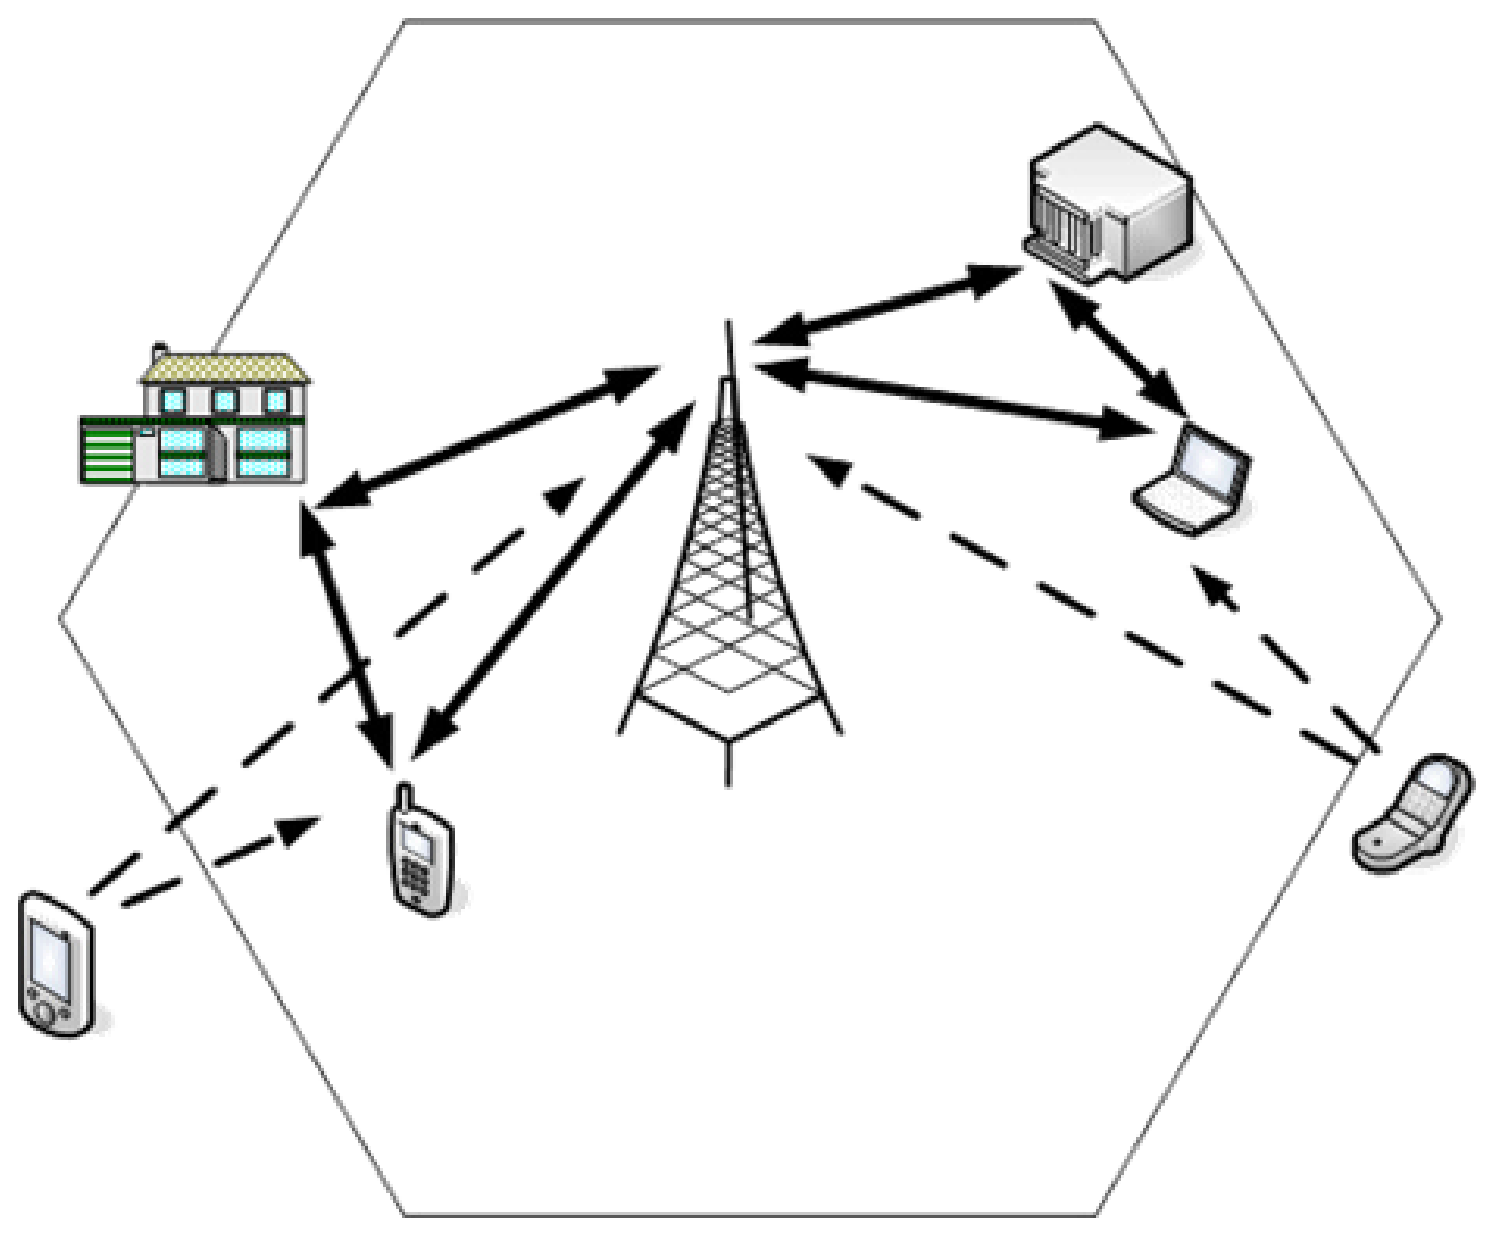
\includegraphics[width=3in]{CDMA_grouplinks.eps}
\caption{ In-cell signals and out-of-cell interferences.}
}\label{CDMA_grouplinks}
\end{figure}


\subsection{Group Blind Multiuser Detection For Forward Link}
In CDMA system, each active mobile station may need communication
with the base station using multiple physical channels which are
generated using different spreading sequences. For example, the
base station want to increase the forward-link data rate for some
users. This can be done using multiple traffic channel for each
user. Or, in some statuses, a mobile station need detect not only
traffic channel(s) but also some signal or control channel(s). At
this time, this mobile station normally knows multiple in-use
spreading sequences for its forward channels while having no
knowledge of the rest channels. At this time, we construct a
$L\times M$ group blind spreading sequence matrix $\bcS$ which is
defined by

\begin{equation}
\begin{array}{rcl}
\bcS&=&[\matrix{\bar{\bs}_1&\bar{\bs}_2&\bar{\bs}_3&\ldots&\bar{\bs}_M}]\\
 &=&[\matrix{\bs_1&\bs_{2}&\ldots&\bs_{g}&{\br}_{1}&{\br}_{2}&\ldots&{\br}_{M-g}}]\\
 &=&\left[\matrix{\bS\bE_g&\bS{\bar\bb}_1&\bS{\bar\bb}_2&\ldots&\bS{\bar\bb}_{M-1}}\right] + {\bN}\\
 &=&\bS\left[\matrix{\bE_g&{\bar\bb}_1&{\bar\bb}_2&\ldots&{\bar\bb}_{M-1}}\right] + {\bN}\\
 &=&\bS\left[\matrix{\bE_g & \bD }\right] + {\bN}\\
 &=&\bS\bB + {\bN}
\end{array} \label{S_FL_g}
\end{equation}

\noindent where $\bs_i$, $i=1,\ 2,\ \ldots,\ g$ are $g$ known
spreading sequences in the group $\cal G$, ${\br}_j$ is a
previously received independent vectors and the $K\times 1$ vector
${\bar\bb}_i=\left[\matrix{A_1b_1[i] & A_2b_2[i]& \ldots &
A_Kb_K[i]}\right]^{\rm T} = \bA\bb_i $ is the corresponding
information vector for all $K$ users, $j=1,\ 2,\ \ldots,\ M-g$,
$M\geq K$, $\bD = [\bar{\bD}^{\rm T}\ \tilde{\bD}^{\rm T}]^{\rm
T}$ and the $g\times (M-1)$ vector $\bar{\bD}$ is the known bit
matrix previously sent for the $1$st user, ${\bN}=[\mathbf{0}\
\tilde{\bN}]$ is a new noise matrix where the first column is a
zero vector and other columns are AWGN vectors with the same
distribution,

\begin{equation}
\begin{array}{rcl}
 \bB&=&\left[\matrix{\bE_g & \bD }\right]\\
  &=&\left[\matrix{\bG_g \cr \matrix{\mathbf{0}& \tilde{\bD}}
 }\right]\\
 &=&\left[\matrix{\bE_g & \matrix{ \bar{\bD}\cr\tilde{\bD}} }\right]\\
 &=&\left[\matrix{\bI_g& \bar\bD \cr \mathbf{0}& \tilde{\bD}
 }\right]

\end{array}\label{B_g}
\end{equation}

\noindent is the information matrix associated with the blind
spreading sequence matrix $\bcS$. $\bG_g = \left[\matrix{\bI_g&
\bar\bD}\right]$ is a known bit matrix to the $1$st user,
$\mbox{rank}\{\tilde{\bD}\}=K-1$ and $\mbox{rank}\{\bB\}=K$.

Combining (\ref{r}) and (\ref{S_FL_g}), the received signal vector
$\br$ can be expressed as

\begin{equation}
\begin{array}{rcl}
\br&=&\bS\bA\bb + \bn\\
 &=&\bS\bB\bB^{+}\bar\bb + \bn\\
 &=&(\bcS-{\bN})\bB^{+}\bar\bb + \bn\\
 &=&\bcS\bB^{+}
 \bar\bb - {\bN}\bB^{+}\bar\bb + \bn\\
 &=&\bcS\bbf + \bar{\bn} \label{rn_g_FL}
\end{array}
\end{equation}

\noindent where $\bar\bb =\bA\bb= \left[A_1b_1[n]\ A_2b_2[n]\
\ldots\ A_Kb_K[n]\right]^{\rm T} = \left[\bA_g\bb_g^{\rm T}\
\tilde{\bb}^{\rm T}\right]^{\rm T}$, $\bB^{+} $ is the
Moore-Penrose matrix inverse of $\bB$ and $\bbf$ is termed the $K
\times 1$ detection vector defined by

\begin{equation}
\begin{array}{rcl}
\bbf&=&\left[\matrix{\bar\bbf\cr\tilde{\bbf}}\right]\\
 &=&\bB^{+}\bar\bb\\
 &=&\left[\matrix{\bE_g&\bD}\right]^{+}\bar\bb\\
 &=&\left[\matrix{\bI_g&\bar{\bD}\cr\mathbf{0}&\tilde{\bD}}\right]^{+}\left[\matrix{\bA_g\bb_g\cr\tilde{\bb}}\right]\
 .
\end{array} \label{DetectorVector_g_FL}
\end{equation}

It is very straightforward to prove that the bits vector $\bb_g$
sent by a group known users at the time $t=n$ can be estimated
using the following conclusion.

\begin{lemma}
The bit vector $\bb_g$ sent for the group of user $\cal G$ at the
time interval $t=n$ can be detected by

\begin{equation}
\begin{array}{rcl}
\hat{\bb}_g&=&\mbox{sign}\left\{\hat{\bA}_g\hat{\bb}_g\right\}\\
&=&\mbox{sign}\left\{\bG_g\bbf\right\}
\end{array}\label{bb_g_estimate}
\end{equation}

\end{lemma}


\begin{proof}

At first, $\bb_g$ can be estimated by
\begin{equation}
\begin{array}{rcl}
\hat{\bb}_g&=&\mbox{sign}\left\{\bA_g\bb_g-{\bar{\bD}}\tilde{\bD}^{+}\tilde{\bb}+{\bar{\bD}}\tilde{\bD}^{+}\tilde{\bb}\right\}\\
&=&
\mbox{sign}\left\{\left[\matrix{\bI_g&{\bar\bD}}\right]\left[\matrix{\bA_g\bb_g-{\bar\bD}\tilde{\bD}^{+}\tilde{\bb}\cr\tilde{\bD}^{+}\tilde{\bb}}\right]\right\}\\
&=& \mbox{sign}\left\{\bG_g\left[\matrix{\bI_g&-{\bar\bD}\tilde{\bD}^{+}\cr\bzero&\tilde{\bD}^{+}}\right]\left[\matrix{\bA_g\bb_g\cr\tilde{\bb}}\right]\right\}\\
&=&
\mbox{sign}\left\{\bG_g\left[\matrix{\bI_g&-{\bar\bD}\tilde{\bD}^{+}\cr\bzero&\tilde{\bD}^{+}}\right]\bar\bb\right\}
\end{array}\label{bb1_g}
\end{equation}


\noindent On the other hand, with (\ref{B_asynch}), we know that

\begin{equation}
\bB\left[\bE_g\
\matrix{-{\bar\bD}\tilde{\bD}^+\cr\tilde{\bD}^+}\right]\bB
=\left[\matrix{\bI_g&{\bar\bD}\cr\bzero&\tilde{\bD}}\right]\left[\matrix{\bI_g&-{\bar\bD}\tilde{\bD}^+\cr\bzero&\tilde{\bD}^+}\right]\left[\matrix{\bI_g&{\bar\bD}\cr\bzero&\tilde{\bD}}\right]
=\bB\ . \label{psedoB1_g}
\end{equation}

\noindent So, the Moore-Penrose Matrix inverse $\bB^{+}$ of $\bB$
can be written by

\begin{equation}
\bB^{+}
=\left[\matrix{\bI_g&-{\bar\bD}\tilde{\bD}^+\cr\bzero&\tilde{\bD}^+}\right]\
. \label{psedoB2_g}
\end{equation}


\noindent Using (\ref{B_g}) and (\ref{psedoB2_g}), (\ref{bb1_g})
can be re-written by

\begin{equation}
\begin{array}{rcl}
\hat{\bb}_g&=& \mbox{sign}\left\{\bG_g\bB^{+}\bb\right\}\\
&=& \mbox{sign}\left\{\bG_g\bbf\right\}\\
\end{array}
\end{equation}

\noindent and the detection vector $\bbf$ can also be re-written
by

\begin{equation}
\begin{array}{rcl}
\bbf&=&\left[\matrix{\bA_g\bb_g-{\bar\bD}\tilde{\bD}^{+}\tilde{\bb}\cr\tilde{\bD}^{+}\tilde{\bb}}\right]
\end{array} \label{DetectorVector2_g_FL}
\end{equation}


This lemma is then proven.
\end{proof}

\subsection{Group Blind Multiuser Detection For Reverse Link}
At this time, we construct a $L\times M$ asynchronous group blind
spreading sequence matrix $\bcS$ which is defined by

\begin{equation}
\begin{array}{rcl}
\bcS&=&[\matrix{\bar{\bs}_1&\bar{\bs}_2&\bar{\bs}_3&\ldots&\bar{\bs}_M}]\\
 &=&[\matrix{\bs_1&\bs_{2-}&\bs_{2+}&\ldots&\bs_{g-}&\bs_{g+}&\ldots&\bs_{g}&{\br}_{1}&{\br}_{2}&\ldots&{\br}_{M-2g+1}}]\\
 &=&\left[\matrix{\bS\bE_g&\bS{\bar\bb}_1&\bS{\bar\bb}_2&\ldots&\bS{\bar\bb}_{M-1}}\right] + {\bN}\\
 &=&\bS\left[\matrix{\bE_g&{\bar\bb}_1&{\bar\bb}_2&\ldots&{\bar\bb}_{M-1}}\right] + {\bN}\\
 &=&\bS\left[\matrix{\bE_g & \bD }\right] + {\bN}\\
 &=&\bS\bB + {\bN}
\end{array} \label{S_RL_g}
\end{equation}

\noindent where $\bs_i$, $i=1,\ 2,\ \ldots,\ g$ are $g$ known
group spreading sequences, ${\br}_j$, $j=1,\ 2,\ \ldots,\ M-g$,
are $M-g$ previously received independent vectors and the $K\times
1$ vector ${\bar\bb}_i=\left[\matrix{A_1b_1[i] & A_2b_2[i]& \ldots
& A_Kb_K[i]}\right]^{\rm T} = \bA\bb_i $ is the corresponding
information vector for all $K$ users, $M\geq K$, $\bD =
[\bar{\bD}^{\rm T}\ \tilde{\bD}^{\rm T}]^{\rm T}$ and the $g\times
(M-1)$ vector $\bar{\bD}$ is the known bit matrix previously sent
for the $1$st user, ${\bN}=[\mathbf{0}\ \tilde{\bN}]$ is a new
noise matrix where the first column is a zero vector and other
columns are AWGN vectors with the same distribution,

\begin{equation}
\begin{array}{rcl}
 \bB&=&\left[\matrix{\bE_g & \bD }\right]\\
  &=&\left[\matrix{\bG_g \cr \matrix{\mathbf{0}& \tilde{\bD}}
 }\right]\\
 &=&\left[\matrix{\bE_g & \matrix{ \bar{\bD}\cr\tilde{\bD}} }\right]\\
 &=&\left[\matrix{\bI_g& \bar\bD \cr \mathbf{0}& \tilde{\bD}
 }\right]

\end{array}\label{B_RL_g}
\end{equation}

\noindent is the information matrix associated with the blind
spreading sequence matrix $\bcS$. $\bG_g = \left[\matrix{\bI_g&
\bar\bD}\right]$ is a known bit matrix to the $1$st user,
$\mbox{rank}\{\tilde{\bD}\}=K-1$ and $\mbox{rank}\{\bB\}=K$.

Combining (\ref{r}) and (\ref{S_RL_g}), the received signal vector
$\br$ can be expressed as

\begin{equation}
\begin{array}{rcl}
\br&=&\bS\bA\bb + \bn\\
 &=&\bS\bB\bB^{+}\bar\bb + \bn\\
 &=&(\bcS-{\bN})\bB^{+}\bar\bb + \bn\\
 &=&\bcS\bB^{+}
 \bar\bb - {\bN}\bB^{+}\bar\bb + \bn\\
 &=&\bcS\bbf + \bar{\bn} \label{rn_g_RL}
\end{array}
\end{equation}

\noindent where $\bar\bb =\bA\bb= \left[A_1b_1[n]\ A_2b_2[n]\
\ldots\ A_Kb_K[n]\right]^{\rm T} = \left[\bA_g\bb_g^{\rm T}\
\tilde{\bb}^{\rm T}\right]^{\rm T}$, $\bB^{+} $ is the
Moore-Penrose matrix inverse of $\bB$ and $\bbf$ is termed the $K
\times 1$ detection vector defined by

\begin{equation}
\begin{array}{rcl}
\bbf&=&\left[\matrix{\bar\bbf\cr\tilde{\bbf}}\right]\\
 &=&\bB^{+}\bar\bb\\
 &=&\left[\matrix{\bE_g&\bD}\right]^{+}\bar\bb\\
 &=&\left[\matrix{\bI_g&\bar{\bD}\cr\mathbf{0}&\tilde{\bD}}\right]^{+}\left[\matrix{\bA_g\bb_g\cr\tilde{\bb}}\right]\
 .
\end{array} \label{DetectorVector_g_RL}
\end{equation}


\pagebreak

\section{Initial Setup And Adaptivity}

\begin{figure}
\center{
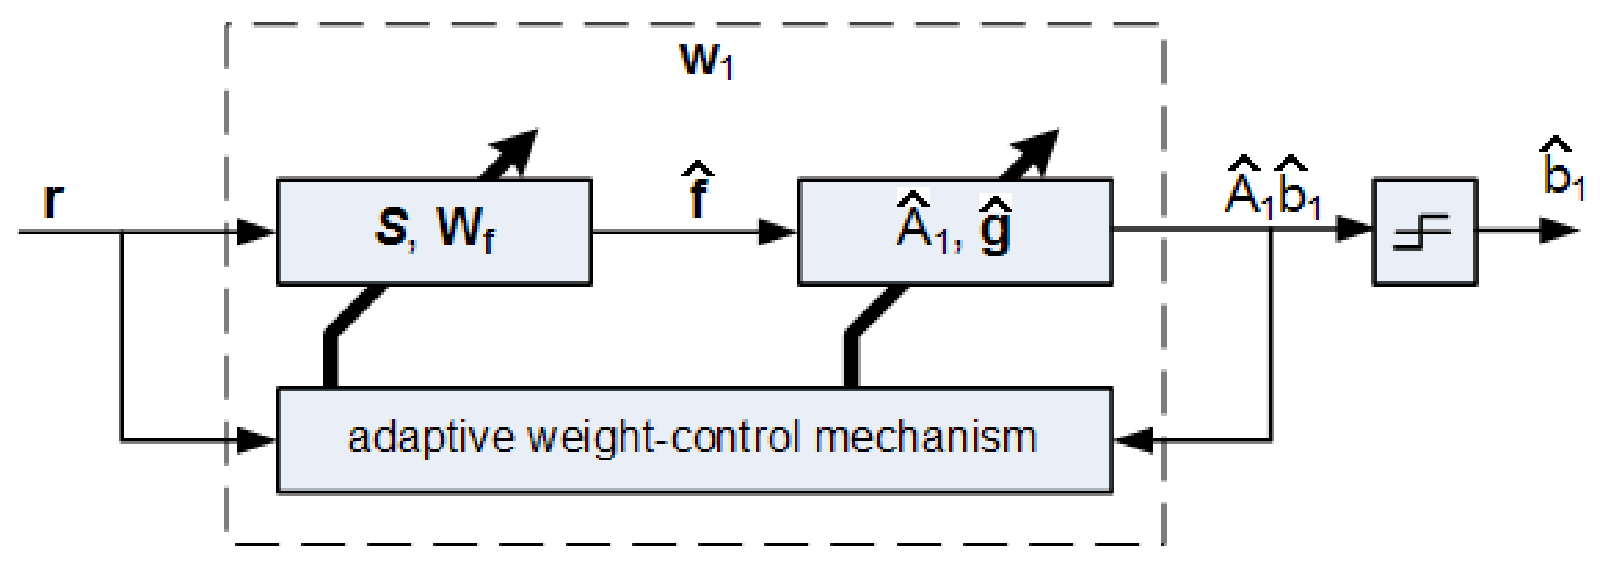
\includegraphics[width=5.5in]{BMUD_structure7.eps}
\caption{ The proposed adaptive blind multiuser detection
structure.} }\label{AMUDstruct}
\end{figure}

With the proposed blind multiuser detection framework expressed in
(\ref{b_estimation}) and (\ref{A_estimation}), the two key
components in the linear blind multiuser detector $\bw_{1}$ are
the detection vector $\bbf$ and the detected bit vector
$\bg$~\footnote{Without loss of the generality, we only consider
$M=1$ case here. }. Obviously the accuracy of estimating $\bbf$
and $\bg$ determines the performance of detecting $\hat{b}_1$,
especially when the multiuser channels are experiencing various
fading and distortions. Hence, it is necessary to looking for a
efficient adaptive mechanism for continuously updating
$\hat{\bbf}$ and $\hat{\bg}$, which can be illustrated in
Fig.~\ref{AMUDstruct}. On the other hand, though it looks similar
to the conventional one-step decorrelating detection, the proposed
framework actually utilizes and depends on the $M-1$ previously
estimated bits. There possibly exists an error propagation
problem. This makes how to initialize the first at least $M-1$
detections unignorable.

\subsection{Adaptive Updating}

With (\ref{w_LS}), (\ref{w_TLS}), (\ref{w_MLS}), (\ref{w_BLU}) and
(\ref{w_MSE}), we can see that the updating of $\bW_{\bbf}$ and
$\hat{\bg}$ actually is determined by how to construct $\bcS$ and
how to estimate $A_1$. These two questions sound similar to a
general equalization problem. However, the difference is that the
model proposed in (\ref{S_0}) and (\ref{r_blind}) is memoryless
while equalization is normally used for handling memory channels
with inter-symbol interference (ISI). Therefore, we can use a
selective scheme for constructing $\bcS$. If we can pretty sure
which estimates of $A_1b_1$ is not accurate enough, we can update
the next $\bcS$ only with the $\br$ corresponding to a good
$A_1b_1$ estimate. For $A_1$ estimation, the popular adaptive
signal estimation schemes, such as LMS and RLS, can be easily
applicable here.


\subsection{Initial Setup}

Initial setup can always be a problem with blind detection or
estimation schemes. There are normally two popular approaches. One
is to use a explicit pilot channel which can help blind receiver
achieve fast and accurate convergence. The another approach is a
completely blind approach where the receiver will take care of all
necessary estimations. Blind initial setup procedures will
normally take more time or steps than pilot assistant schemes.

\pagebreak

\section{Performance Analysis}

\subsection{Geometric Interpolation}

It is known that the classic decorrelating detector actually
performs the following operation.

\begin{equation}
\begin{array}{rcl}
\hat\bb&=&\mbox{sign}\{\bW_{\rm DD}^{\rm T}\br\}\\
 &=&\mbox{sign}\{\bS^+\br\}
\end{array}
\end{equation}

\noindent where $\bW_{\rm DD}$ is the linear filter representation
of the decorrelating detector bank and the $K\times L$ matrix
$\bS^+$ is the Moore-Penrose generalized inverse of $\bS$.
In~\cite{Elda02}, it is shown that each of the above decorrelating
detectors is the \em oblique projection\rm\ of the desired user's
signature vector onto the orthogonal complement of the space
spanned by other users' signature vectors along the orthogonal
complement of this space spanned by this user's vector. For
example, the decorrelating detector $\bw_{\rm DD1}$ for the first
user is


\begin{equation}
\begin{array}{rcl}
\bw_{\rm DD1}&=&\bP_1^{\angle}\bs_1\\
 &=&{1 \over \bs_1^{\rm T}\bP_1^{\perp}\bs_1 }\bP_1^{\perp}\bs_1
\end{array}
\end{equation}

\noindent where $\bP_1^{\angle}$ denotes the oblique projection of
$\bs_1$ and $\bP_1^{\perp}$ is the orthogonal projection for user
1 onto the orthogonal complement, which is denoted by
$\bar{S}_1^{\perp}$, of the subspace
$\bar{S}_1=\mbox{span}\{\bs_k\ |\ k\neq 1\}$  and ${S}_1^{\perp}$
denotes the orthogonal complement of the subspace
$S_1=\mbox{span}\{\bs_1\}$. This can be illustrated in
Fig.~\ref{DD_geometric}. The linear filter representation of the
proposed LS estimation of user 1's $\bbf$ in (\ref{f_LS}) can
therefore be taken as the oblique projection of $\bs_1$ onto the
orthogonal complement $\bar{\cal S}_{1}^{\perp}$ of the space
$\bar{\cal S}_{1}$, where

\begin{equation}
\begin{array}{rcl}
\bar{\cal S}_{1}& =& \mbox{span}\left\{\bar\br_m\ |\ 1\leq m\leq
M-1\right\}
\end{array}
\end{equation}

\noindent and

\begin{equation}
\begin{array}{rcl}
\bar{\cal S}_{1}^{\perp}& =& \left\{\bv\ |\ \bv^{\rm T}\bu=0,\
\forall\bu\in\bar{\cal S}_{1} \right\}
\end{array}.
\end{equation}


\begin{figure}
\center{
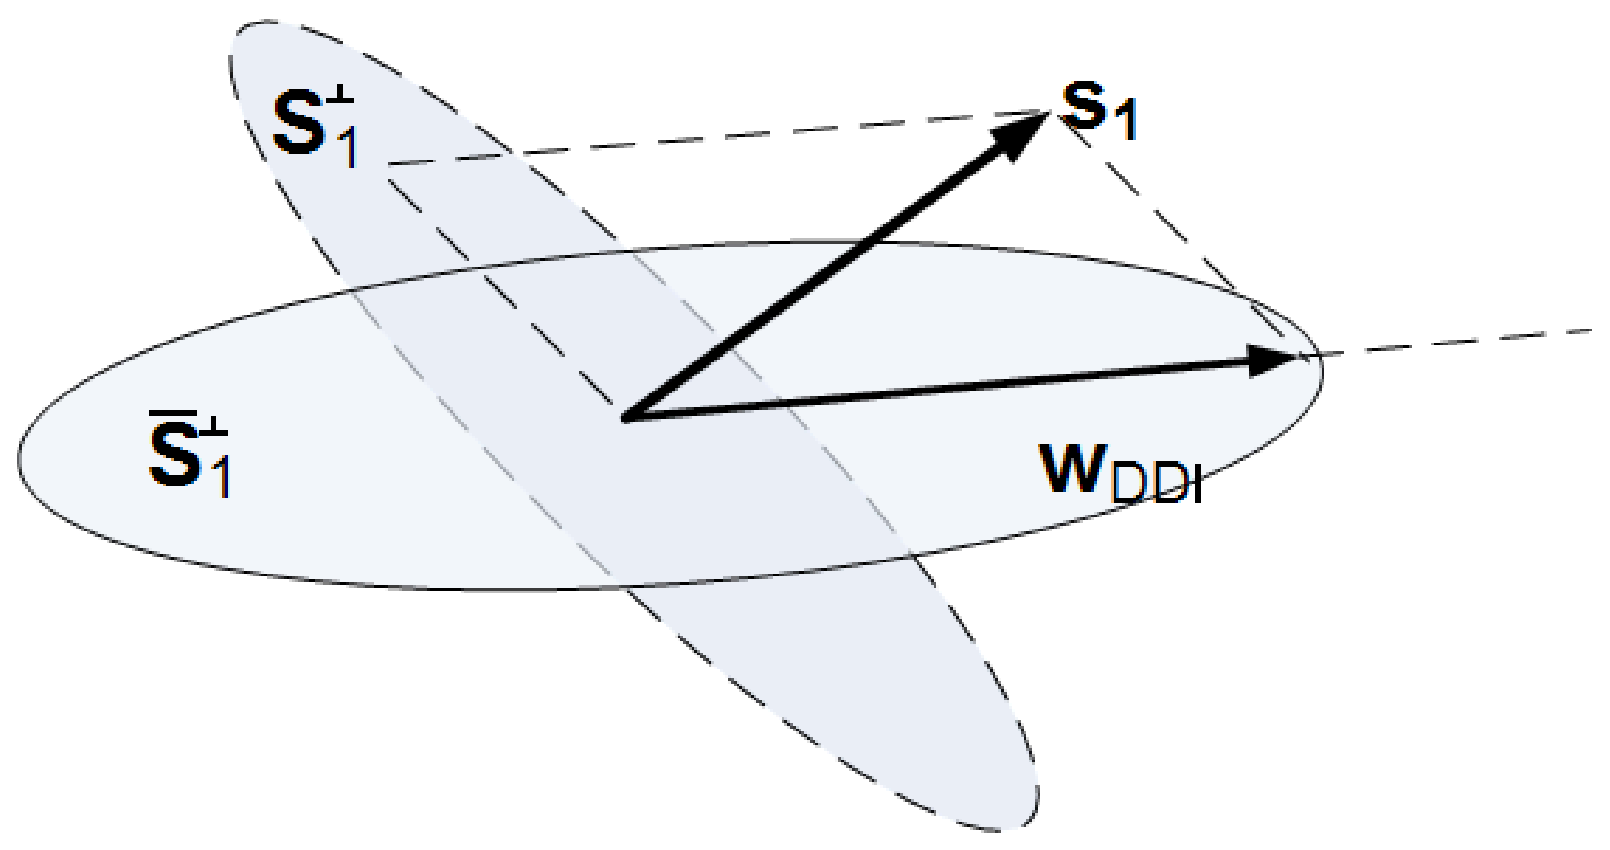
\includegraphics[width=3in]{DD_geometric.eps}
\caption{ The geometric interpretation of decorrelating detector.}
}\label{DD_geometric}
\end{figure}



\subsection{Cram\'{e}r-Rao Lower Bound (CRLB)}

The CRLB is given by the inverse of the Fisher information matrix
(FIM). Providing the blind spreading matrix $\bcS$ is known
beforehand, we first define the parameter vector $\mathbf{\phi} =
\left[\bar{\sigma}^{2}\ \bbf^{\rm T}\right]^{\rm T}$, where
$\bar{\sigma}^{2} =(1+\frac{M-1}{M-K})\sigma^{2}$ is the variance
of elements in $\bar\bn$ for computing the FIM, which is defined
by

\begin{equation}
\begin{array}{rcccl}
{\rm FIM}&=&{\rm CRLB}^{-1}\left(\mathbf{\phi}\ |\ \bcS\right) &
=& {\rm E} \left\{ \left( \frac{\partial \ln{\cal L}}{\partial
\mathbf{\phi}} \right) \left( \frac{\partial \ln{\cal L}}{\partial
\mathbf{\phi}} \right)^{\rm H} \right\} \label{fim}
\end{array}
\end{equation}

\noindent where $\ln{\cal L}$ is the log-likelihood function given
by

\begin{equation}
\begin{array}{rcl}
\ln{\cal L}&=&C-L\ln\bar{\sigma}^2-\frac{1}{2\bar{\sigma}^2}\parallel\br-\bcS\bbf\parallel_2^2\\
&=&C-L\ln\bar{\sigma}^2-\frac{1}{2\bar{\sigma}^2}\parallel\mathbf{e}\parallel_2^2
\end{array}\label{logl}
\end{equation}

\noindent where $C$ is a constant and $\mathbf{e}=\br-\bcS\bbf$.

The derivatives of the log-likelihood function can be calculated
with respected to $\bar{\sigma}^2$ and $\bbf$. These first-order
partial differences of the log-likelihood function are


\begin{equation}
\begin{array}{rcl}
\displaystyle{\partial\ln{\cal
L}\over\partial\bar{\sigma}^2}&=&-\displaystyle{L\over\bar{\sigma}^2}+\displaystyle{2\over\bar{\sigma}^4}\parallel\mathbf{e}\parallel_2^2
\end{array}
\end{equation}

\begin{equation}
\begin{array}{rcl}
\displaystyle{\partial\ln{\cal
L}\over\partial\bbf}&=&\displaystyle{1\over\bar{\sigma}^2}\bcS^{\rm
T}\mathbf{e}
\end{array}.
\end{equation}

\noindent with the above derivatives, we can obtain

\begin{equation}
\begin{array}{rcl}
{\rm E}\left\{\left(\displaystyle{\partial\ln{\cal
L}\over\partial\bar{\sigma}^2}\right)\left(\displaystyle{\partial\ln{\cal
L}\over\partial\bar{\sigma}^2}\right)^{\rm
T}\right\}&=&\displaystyle{L\over\bar{\sigma}^4}
\end{array}
\end{equation}

\begin{equation}
\begin{array}{rcl}
{\rm E}\left\{\left(\displaystyle{\partial\ln{\cal
L}\over\partial\bbf}\right)\left(\displaystyle{\partial\ln{\cal
L}\over\partial\bbf}\right)^{\rm
T}\right\}&=&\displaystyle{1\over\bar{\sigma}^2}\bcS^{\rm T}\bcS
\end{array}
\end{equation}


After some calculations, it can be shown that the CRLB for the
parameters of interest ($\bar{\sigma}^2$ and $\bbf$) are


\begin{equation}
\begin{array}{rcl}
{\rm CRLB}^{-1}\left(\mathbf{\phi}\ |\ \bcS\right) & =& {\rm E}
\left\{ \left( \frac{\partial \ln{\cal L}}{\partial \mathbf{\phi}}
\right) \left( \frac{\partial
\ln{\cal L}}{\partial \mathbf{\phi}} \right)^{\rm T} \right\}\\
&=&\left[\matrix{\displaystyle{L\over\bar{\sigma}^4}&\cr&\displaystyle{1\over\bar{\sigma}^2}\bcS^{\rm
T}\bcS}\right]
\end{array}
\end{equation}

\noindent Therefore, proving $\bcS$ is known, the closed-form CRLB
expression of $\bbf$ is given by

\begin{equation}
\begin{array}{rcl}
{\rm CRLB}(\bbf\ |\ \bcS) & =&\bar{\sigma}^2(\bcS^{\rm
T}\bcS)^{\rm +}
\end{array}
\end{equation}



\pagebreak

\section{Computer Simulations}
\pagebreak

\section{Conclusions}
\pagebreak
\bibliographystyle{unsrt}
\bibliography{FastBDD}

\end{document}
